\documentclass[conference]{IEEEtran}
\IEEEoverridecommandlockouts
% The preceding line is only needed to identify funding in the first footnote. If that is unneeded, please comment it out.
\usepackage{cite}
\usepackage{amsmath,amssymb,amsfonts}
\usepackage{algorithmic}
\usepackage{graphicx}
\usepackage{textcomp}
\usepackage{xcolor}
\def\BibTeX{{\rm B\kern-.05em{\sc i\kern-.025em b}\kern-.08em
    T\kern-.1667em\lower.7ex\hbox{E}\kern-.125emX}}
\begin{document}

\title{Recycling Assistant\\
{\footnotesize \textsuperscript{}Identifying and Categorizing Objects based on Recyclability}
}

\author{\IEEEauthorblockN{Doo Woong Chung}
\IEEEauthorblockA{\textit{Dept. Information Systems} \\
\textit{Hanyang University}\\
Seoul, South Korea \\
dwchung@hanyang.ac.kr}
\and
\IEEEauthorblockN{Kim Soohyun}
\IEEEauthorblockA{\textit{Dept. Information Systems} \\
\textit{Hanyang University}\\
Seoul, South Korea \\
soowithwoo@gmail.com}
\and
\IEEEauthorblockN{Lim Hongrok}
\IEEEauthorblockA{\textit{Dept. Information Systems} \\
\textit{Hanyang University}\\
Seoul, South Korea \\
hongrr123@gmail.com}
}

\maketitle

\begin{abstract}
Sometimes being able to correctly identify and understand how to recycle certain items can be difficult. As such, the Recycling Assistant hopes to be able to alleviate some of those questions, via the identification and categorization of more common objects.

An observation that can be made is that certain recyclable items are not often disposed of an in efficient manner - such as plastic bottles not being emptied of air - causing a lot of empty volume. As a result, an additional feature that the Recycling Assistant hopes to implement is notifying the user when an item can be disposed of in a more optimal manner.
\end{abstract}

\begin{IEEEkeywords}
identification, detection, classification, opencv, recycling, waste
\end{IEEEkeywords}

\section{Role Assignments}
Below is the table of external role assignments for this project. Due to the small team size, the development manager position has been split between the software developers, in order to facilitate quick decision making.
\newline

\begin{table}[htbp!]\normalsize
\begin{center}
\begin{tabular}{|p{1.5cm}|p{1.7cm}|p{4.5cm}|}
\hline
\textbf{Name} & \textbf{\textit{Role}}& \textbf{\textit{Responsibilities}}\\
\hline
Doo Woong Chung & Co-Development Manager \& Software Developer &
Responsible for assigning tasks and identifying the next step in the project/what needs to be done to stay on track, and converting requirements into tangible functionality. In addition, they are also responsible for identifying frameworks that would work best with the project.\newline
\newline Responsible for implementing software functionality and collaborating with other Software Developers in order to fulfill and push required features. Also responsible for maintaining code and coordinating pull requests.
\\ \hline
\end{tabular}
\label{tab1}
\end{center}
\end{table}
\newpage

\begin{table}[htbp!]\normalsize
\begin{center}
\begin{tabular}{|p{1.5cm}|p{1.7cm}|p{4.5cm}|}
\hline
\textbf{Name} & \textbf{\textit{Role}}& \textbf{\textit{Responsibilities}}\\
\hline
Kim Soohyun & User \& Customer &
Responsible for testing the application, and pointing out any flaws in the application that may requirement improvement.\newline
\newline In addition, they are responsible for providing feedback in how to improve upon those flaws in order, as well as continuously checking off on whether the requirements are being fulfilled. 
\newline In the event that the requirements do not seem to be fulfilled at a reasonable level, they are responsible for relaying actionable feedback, and evaluating implemented features.
\\ \hline
Lim Hongrok & Co-Development Manager \& Software Developer &
Responsible for implementing software functionality and collaborating with other Software Developers in order to fulfill and push required features.\newline
\newline In addition, they are responsible for keeping things grounded, and making sure that the minimum viable product is on track. 
\newline They are also responsible for communicating with the user and customer to receive and incorporate feedback into the product. Also responsible for maintaining code and coordinating pull requests.
\\ \hline
\end{tabular}
\label{tab1}
\end{center}
\end{table}

\newpage

\section{Introduction}
\subsection{Problem Statement}
The Recycling Assistant is a project hoping to identify, and categorize recyclable materials. In this form, we envision the Recycling Assistant to allow the user to hold up an item and display which category of recycling the item belongs in. In the event that the item is not recyclable, it will notify the user accordingly. In addition, if there is an additional tip for that category (ie. detected bottle) it will notify the user that an optimal method of recycling the item would be to minimize its volume (crushing it). \\
Recycling can be a convoluted topic at times, with people sometimes confusing what is recyclable and what is not. As a result, objects are often incorrectly disposed of, with either recyclables ending up in general waste, or objects that aren't recyclable, heading to the recycling plant. For example, hybrid materials is often the case, or confusion regarding the actual material of the object. This leads to only a fraction of the submitted recycled waste actually being able to be recycled, with the remainder heading back to landfills. \\

Our goal is to provide an assistant program that can quickly guide the user to which type of category of recycling the item that the user shows the camera, belongs in - if it is recyclable to begin with. Otherwise, they will be notified that it is more fitted to general waste, or unknown. This would help cut down on the issue of the user either not being sure of whether the object is recyclable and disposing of it in general waste, as well as help provide the user with helpful tips on how to optimize their recycle behavior.\\
We hope to also be able to incorporate the detection of different materials in a way such that the Assistant can differentiate between several types of material on the same object, and inform the user on why the object would not be recyclable in its current state (ie. Plastic film on a paper box is detected).\\

\subsection{Motivation}

The idea for this project stems from the observation that recycling, while seemingly a simple topic from an external point of view, can get confusing with certain types of objects. For example, as a mixture of different materials are often used in products these days, it is sometimes confusing to tell if an object is really recyclable or not. \\
In addition, as AI/ML usage in environmentally friendly initiatives is a topic of high interest, waste-related datasets are plentiful, and we hope to leverage these datasets in order to train something that would help users with a quick and easy way to optimize their recycling behavior, while also providing useful statistics.\\

While there are a fair amount of similar, existing projects, they are targeted towards commercial/industrial applications, and are typically not open source. Thus, we were motivated to provide an open-source alternative application for users to be able to run themselves.\\

Our application focuses on providing people with the convenience of being able to quickly consult with the application and receive feedback on how an object is classified in terms of recyclability, in addition to receiving any potential tips to with regards to their disposal patterns. \\
As a result, we hope that this application will help reduce the problem of incorrectly recycled objects occurring, or recyclable objects being sent to the landfill from a normal consumer user standpoint. \\~\\

\section{Existing Products}

There are quite a bit of related existing products for this Recycling related AI work, as it is a field of interest in both the AI sector, as well as having a positive environmental affect. However, they generally range from proprietary solutions, or projects that are not open source.

In general, they seem to generally be integrated into specialized commercial applications, or proof of concepts.
\newline

\subsection{Recycle Mate \textsuperscript{[1]}}

An Android/iOS application which scans an item, and identifies which bin it goes into. It is highly localized, directing users into the correct bin to dispose of based on information provided by the local council - thus, it is limited to residents in New South Wales only. It takes a picture of the item, analyzes it and directs the user to which color bin it needs to be disposed of in.

Recycle Mate is not open source, and often receives feedback that the picture system is clunky, as well as unhelpful to residents residing outside of New South Wales.
\newline

\subsection{Bin-e Smart Waste Bin \textsuperscript{[2]}}

A "Smart Recycling Bin", which automatically sorts the inserted item into the correct bin. It uses an inserted camera alongside object recognition in order to correctly sort the item. It is described as an "IOT device which sorts and compresses the recyclables automatically, combining unique AI-based object recognition..."

In a sense, Bin-e's system works similarly to what we are looking to achieve, aside from the IOT device integration.
\newline

\subsection{World Waste Platform \textsuperscript{[3]}}

The "Let's Do It AI Project" is a project developed in conjunction with the Let's Do It Foundation and SIFR in partnership with Microsoft. It detects trash, but does not classify between whether or not an item is recyclable, as it is focused purely on identifying litter from the landscape. 

It is open source, and shares information regarding their experience with live image recognition on their blog.
\newline

\subsection{TrashBot \textsuperscript{[4]}}

An industrial and commercial application of AI trash sorting, TrashBot identifies if an object inserted into the TrashBot Smart Bin is recyclable, compost-able or belongs in the landfill. It is intended for use in industrial automation, separating recyclables from landfill waste. 
\newline

\subsection{Greyparrot \textsuperscript{[5]}}

Another industrial approach to waste recognition, Greyparrot uses AI to recognize and classify waste composition at an industrial level - focusing on identifying waste passing through a camera on a conveyor belt.

Based on their released media, it appears to be more detailed than TrashBot, with the ability of distinguishing between types of plastic objects (ie. PET bottles vs plastic tubs).
\newline

\subsection{Intuitive AI \textsuperscript{[6]}}

A similar approach, the Intuitive AI uses computer vision and machine learning to identify the item the user is holding, and tell them which category of recycling it misses - alongside the novelty of yelling at the user if they recycle incorrectly or praising the user if they do it correctly.
\newline

\begin{thebibliography}{00}
\bibitem{b1} “Recycle Mate.” Recycle Mate, https://recyclemate.com.au/. 
\bibitem{b2} “Bin-e Smart Waste Bin.” Bin-e, https://www.bine.world/. 
\bibitem{b3} "World Waste Platform." Let's Do It AI Project, https://ai.letsdoitworld.org/
\bibitem{b4} "TrashBot." CleanRobotics, https://cleanrobotics.com/trashbot/
\bibitem{b5} "Greyparrot AI." Greyparrot, https://www.greyparrot.ai/waste-composition-analysis-software
\bibitem{b5} "Trash-Talking Recycling AI." Nvidia Blogs, https://blogs.nvidia.com/blog/2020/02/03/intuitive-ai-schools-you-on-recycling/
\end{thebibliography}~\\~\\

\section{Requirements Analysis}

\subsection{Opening the Application}
Once the application is started, the user should immediately be presented with a button to begin the session. The session presents with a front-view camera view, alongside other UI elements. If it is the user's first time opening the application, or they do not have a valid settings file, they will be directed to the settings menu referred to in requirement B.1 (Settings Menu).
\newline
\subsection {Settings}

The application should come with a set of default or baseline settings, that the user should be able to edit via a set settings context menu button.
\newline
\begin{itemize}
\item{\emph{Settings Menu:}}\\
The settings menu should contain various settings related to the operation of the application, alongside storage of the data, as well as as having the option of disabling certain UI elements. The settings menu should also contain an option for the user to choose a different camera source (ie. manual entry of a network camera).
\newline

\item{\emph{Loading/Storage of Settings:}}\\
When the application starts, the settings should automatically be loaded - with the default being loaded if the current saved data is either corrupted, or not set. 

The settings should be appropriately stored, in a manner that best prevents corruption of the settings data should the application exit in an unintended manner while the application is saving the user's settings. The settings should be saved when the user clicks the "Save Settings" button.
\newline
\end{itemize}

\subsection{Exiting the Application}
The user should be able to exit the application normally, with minimal chance of data corruption. The exit should be smooth, and should aim to exit immediately without interruption or confirmation message.
\newline
\subsection{Input Support}

The application should be able to support a real-time input of a camera, through either a physically connected input, or a local network camera input. In the event that there is no valid input detected, the user should be notified appropriately.
\newline
\subsection{Real Time Analysis}

The application should be able to handle real-time detection, as well as be able to analyze and classify the object based on the input, and  visual output (ie. text and bounding boxes). 
\newline
\subsection{Object Detection}

The application, on successful object detection, should draw a bounding box around the object and output that result. If multiple objects are detected in the frame, they must also be drawn appropriately.
\newline
\subsection{Classification/Categorization}

Based on successful object detection, the user should receive textual feedback on what the detected item's classification/categorization is. For example, if the user holds up a plastic bottle, after detection, the screen should output that it is a detected plastic object.
\newline
\subsection{Additional Statistics - Detection}

After successful object detection, the application should show the confidence level of the inference, alongside detected objects in order to be able to insert it into the database specified in requirement G.
\newline
\subsection{Failure to Classify/Categorize}

In the event that the application is unable to adequately classify/categorize the object (ie. low confidence), it should ignore the object and not cause a detection event.
\newline
\subsection{Local Database}
A local database should be retained in order to save results of previously detected objects. When an object is successfully scanned, data such as the timestamp, detected object, object classification, object categorization, confidence level, picture, should be stored in the database.

This database should also be able to be accessed by the user in order to draw and show additional statistics, such as most frequently detected category, overall confidence level, etc.
\newline
\subsection{Statistics}
Basic statistics should be available, such as the overall detection count, detection count per category, etc. There should also be a separate set of statistics for the session's detections.

A statistics menu should be available via an UI element on the main screen.
\newline
\subsection{Educational Feedback}
The application should be able to add a general explanation to each output, educating the user on why a certain object is not recyclable, or why it is not recyclable in its current state.

\newpage
\section{Role Assignment}

\begin{table}[htbp]
\begin{tabular}{|p{1.5cm}|p{1.5cm}|p{4.7cm}|}
\hline
\textbf{Name} & \textbf{Main Role} & \textbf{Responsibility Description}\\ \hline
Doo Woong Chung & Back-End & 
\newline Handling of the Input/Output system\newline- Implementation of OpenCV into the application, as well as handling the output processing such as text output/bounding boxes.
\newline 
\newline Repository Maintainer\newline- Handling Repository Commits, General Maintenance.
\newline 
\newline General Application Architect\newline- Architect of general systems used in the application, and how they'll link together to form the final product. 
\newline 
\newline Base Application Prototyping\newline- Prototyping with related applications that will be used, such as OpenCV to test integration. \\ \hline

Kim Soohyun & User/Front-End & 
\newline User Interface System\newline- Analysis pertaining to User Experience, and User Interface.
\newline 
\newline Team Lead\newline- Monitoring overall team performance level and maintaining communication.
\newline 
\newline Project Manager\newline- Monitoring overall progress of the project as well as upcoming deadlines.
\newline 
\newline Tech Blog Maintainer\newline- Maintaining the Team's Tech Blog.
\\ \hline

Lim Hongrok & Back-End & 
\newline Handling of the Database and Model related system\newline- Implementation of PostgreSQL into the application, as well as handling the input of data into the DBMS.
\newline 
\newline Model Training, Prototyping and Evaluation\newline- Prototyping the Model, alongside training and evaluating/testing the Model.
\newline 
\newline Amazon Web Services Handler\newline- Handles AWS related matters, such as usage and configuring of Amazon Web Services that may be used in the training of the model, such as SageMaker.
\newline 
\newline QA/Performance Testing\newline- General Quality Assurance Testing, and Performance Testing (ie. Checking whether the model correctly identifies and classifies the object at a reasonable framerate).
\\ \hline
\end{tabular}
\end{table}

\newpage

\section{General Approach}
At its core, the application handles a real-time video input through either connected network camera, or a physically connected camera (eg. USB). Through OpenCV, the application then analyzes the input and draws a bounded box around the identified object based on its stored/frozen model.\\

The application then returns feedback through text on whether the object is recyclable, or belongs in general waste. If the item is recyclable, it returns feedback based on which type of recycling it belongs in alongside the confidence level. In the event that the item is unknown, or does not return a valid result, the application will either direct the user to the general waste, or return feedback that the application is unsure.\\

The model is trained using one of the plentiful provided databases such as the TACO Dataset, as it contains a plethora of COCO formatted annotated images. Although we were initially considering a YOLO or YOLO derivative in order to speedy detection, the World Waste Platform technical blog mentioned that they also tested out a YOLO implementation, but decided to go with R-CNN due to the difference in expected accuracy.\\

Once the item is identified and classified, the timestamp, identification, classification category will be saved to the local database. Though this database will not be normally accessible to the user, it will be designed in such a way that future feature additions or applications may access it and present data.

\begin{table}[htbp]
    \begin{tabular}{|p{2cm}|p{2.9cm}|p{2.9cm}|}
    \hline
    \textbf{Input} & \textbf{Processing} & \textbf{Output}\\ \hline
    Camera Input & Feed Input Blob into Network & Detected Object, Category, Confidence \\ \hline
    \end{tabular}
\end{table}

A separate super-category will be maintained alongside additional tips - for example, to notify the user that it is recommended to peel off the bottle label in the event that a plastic bottle is detected. In essence, the model will output the general object category of the detected object, which will then feed into a loaded map that contains special instruction for each super-category.\\

This data will then be outputted to the user, with the object instance being drawn, alongside confidence level, and the detected category, super-category and special instructions, or advice.

\newpage
\section{Development Environment}
\subsection{OS}
We will mainly be looking to use the Linux platform as the "base" platform, as it is more convenient to develop for, but we will also look to maximize compatibility with other operating systems so that it may be easily ported, if required.
\newline
\subsection{Services}
For services, we are looking to use AWS SageMaker and AWS Elastic File System in order to optimize our training of the model. Outside of this, we are not looking to offload any computation to the Cloud in terms of the application relying on connection to a VPS instance for example.
\newline

\subsection{Languages}
In this application, C++ may act as the "core" language, while Python will be used in order to handle the dataset, and train the model.\\
\begin{quote}
\subsubsection{C++}~\\
We are targeting usage of the language C++ due to developer familiarity, as well familiarity with libraries that may be leveraged for this project. 
As mentioned previously, C++ has a fair amount of available libraries and frameworks that would help conserve time when implementing features into the product.
\end{quote}
\begin{quote}
\subsubsection{Python}~\\
As the project has a focus on using models, and the detection and classification of objects, Python will be used in order to process the dataset, as it has a myriad of tools that can handle that task easily, such as Pandas.
\end{quote}
\begin{quote}
\subsubsection{SQL - PostgreSQL}~\\
To allow the possibility of expansion and to also leave the data accessible, while offloading the data to the disk rather than the memory, PostgreSQL will be used in order to store data from the detections.
\end{quote}~\\

\subsection{Environment Resources}
Though each of our members have different development environments, an example of one of our software development members' development environment would be the following:

\textbf{Allocated VM Resources:}
\begin{itemize}
\item VM OS: Ubuntu 18.04
\begin{itemize}
\item CPU: 4 Cores @ 3.8GHz
\item RAM: 8GB DDR4-3200mhz
\item Storage: 150GB NVMe PCIe3.0x4
\item Display: 256MB - VBoxSVGA
\item Network: Intel 1000 MT Desktop (NAT)
\end{itemize}
\end{itemize}~\\

\textbf{Model Training Environment:}
\begin{itemize}
\item CPU: 4 vCPUs
\item GPU: NVIDIA T4 Tensor GPU
\item RAM: 16GB
\item Storage: 125GB
\item Networking: 25Gbps Peak
\item EBS Bandwidth: 3.5Gbps Peak
\end{itemize}~\\

\subsection{Version Control}
We will be using GitHub in order to handle versioning for the project, as it ties in well with GitHub's provision of services such as GitHub Pages, as well as some of our members already having a GitHub account.

Due to some of our members' relative unfamiliarity with the Git flow, GitKraken may be used as a convenient GUI'd Git tool to help visualize Git actions, and avoid possible Git-related issues.
\newline

\subsection{Estimated Costs}
As the program is mainly built to be run locally, targeting Linux as a base platform, there are virtually no costs associated with the majority of the program, outside of model training-related costs (SageMaker \& EFS).~\\

\textbf{AWS SageMaker:}
\begin{itemize}
\item Hours: ~10 @ \$0.906 per hour
\item Instance: ml.g4dn.xlarge, 4 Instances
\item Estimated: ~(10 * 4) * \$0.906 = \$36.24
\end{itemize}

\textbf{AWS Elastic File System:}
\begin{itemize}
\item 50GB in total, 20\% of which is frequently accessed
\item Estimated ~\$4.39 per month
\end{itemize}~\\

\subsection{Services In Use}
\subsubsection{AWS SageMaker}~\\
SageMaker is an ML integrated platform provided on Amazon Web Services. One of the advantages to use this software is that it provides the accelerated computing resourses. One of the main concerns about our desired model is that there is a large volume of image dataset to train, and the model should be able to provide the various classification results. Due to the compute power of the AWS service, it takes less time to acquire the trained model.\\
Another advantage is that the distributed training is available. Because we can choose how much instances to engage in the training,this feature also reduces the total training time through a parallel processing.
\newline
\subsubsection{AWS Elastic File System}~\\
EFS(Elastic File System) is a cloud storage service of AWS. While the distributed training executes on the cloud, all datasets should be mounted on each instance and be consumed without any concurrent problem, which EFS supports. In addition, its price policy is the number of reading and writing data. As a result, we can efficiently reduce the cost because the total size of required images, including training, validation and augmentation, is quite large, while most of the data remains in "cold storage" during the training.
\newline

\subsection{Software In Use}
We will be looking at leveraging various, and multiple frameworks for this project.\\

\begin{table}[htbp!]\normalsize
\begin{center}
\begin{tabular}{|p{1.5cm}|p{1.5cm}|p{4.7cm}|}
\hline
\textbf{Software} & \textbf{\textit{License}}& \textbf{\textit{Description \& Explanation}}\\
\hline
SSD MobileNet v2 + Tensorflow\textsuperscript{0}\textsuperscript{1} & Apache-2.0 &
SSD MobileNet v2 is an object recognition algorithm that is fast - using a "single shot" to detect multiple objects. This will fit our necessity for speediness, especially once frozen for inference, as we are going for real-time detection. 

We will be following and slightly modifying a guide in order to streamline the process of training and exporting this model.
\\ \hline
OpenCV \textsuperscript{2} & Apache-2.0 &
OpenCV is a software library that focuses on computer vision. It contains support for ML model execution, as well as various image manipulation functions.\newline

A lot of the internal UI features will be implemented via OpenCV (ie. bounding boxes, displaying of results, etc), and the model will be fed to OpenCV's native model handling to return these results. It is available on many platforms and languages, supporting Linux, C++ and Python, amongst many others.
\\ \hline
\end{tabular}
\label{tab1}
\end{center}
\end{table}

\begin{table}[htbp!]\normalsize
\begin{center}
\begin{tabular}{|p{1.5cm}|p{1.5cm}|p{4.7cm}|}
\hline
\textbf{Software} & \textbf{\textit{License}}& \textbf{\textit{Description \& Explanation}}\\
\hline
Qt \textsuperscript{3} & GPL, LGPLv3 &
Qt is described as a "cross-platform application development framework for desktop, embedded and mobile". It is written in C++, and handles C++ code. \newline\newline
Qt will be used in order to implement UI elements in the application. Qt comes complete with a UI designing software, to help the UI building process flow more smoothly.
\\ \hline
PostgreSQL \textsuperscript{4} & PostgreSQL License (Liberal) &
PostgreSQL is an open-source database management system. It is an object-relational database management system, that comes with built-in C language bindings.\newline\newline
PostgreSQL would mainly be used for our database operations - for the storage of both general and debugging data related to user scans.
\\ \hline
libpqxx \textsuperscript{5} & BSD-3 &
libpqxx is the C++ API for PostgreSQL, as a convenient library in order to be able to use C++ in order to establish a database connection instead of the built-in C language bindings.\newline\newline
It is a C++ wrapper for the built-in wrapper for the PostgreSQL standard C bindings (libpq) - it will be used in order to insert data into the PostgreSQL database.
\\ \hline
rapidjson \textsuperscript{6} & MIT/JSON License &
rapidjson is a fast and efficient JSON parser written in C++, with two main styles of parsing/generation - SAX/DOM.\newline\newline
rapidjson will be used in order to handle (read/write) settings and configuration, which will be stored in the JSON format.
\\ \hline
\end{tabular}
\label{tab1}
\end{center}
\end{table}

\begin{thebibliography}{00}
\bibitem{b0} “Training SSD MobileNet v2 with TACO dataset” Bouwe Ceunen, https://www.kaggle.com/bouweceunen/training-ssd-mobilenet-v2-with-taco-dataset/
\bibitem{b1} “Mask-RCNN-Tensorflow” AWS, https://github.com/tensorflow/
\bibitem{b2} “OpenCV” OpenCV, https://github.com/opencv/opencv/
\bibitem{b3} "Qt" Qt, https://www.qt.io/
\bibitem{b4} "PostgreSQL" PostgreSQL, https://www.postgresql.org/
\bibitem{b5} "libpqxx" jtv, https://github.com/jtv/libpqxx/
\bibitem{b6} "rapidjson" Tencent, https://github.com/Tencent/rapidjson/
\end{thebibliography}~\\~\\

\subsection{Styling Guidelines}
\subsubsection{CppCoreGuidelines}
\begin{itemize}
\item https://isocpp.github.io/CppCoreGuidelines/
\end{itemize}~\\
For C++, we will be referring to the CppCoreGuidelines in order to stick to a consistent coding style, as well as avoiding unintended consequences that may arise from, for example, improper pointer handling, as well as avoiding things that may cause bugs that are harder to debug, such as the use of macros.
\newline
\subsubsection{Clang-Tidy}
\begin{itemize}
\item https://clang.llvm.org/extra/clang-tidy/
\end{itemize}~\\
To check whether the code doesn't stray too far from the core guidelines, Clang-Tidy with the CppCoreGuidelines flag will be used to ease the process.~\\

\subsection{Dataset}
\subsubsection{TACO}
\begin{itemize}
\item http://tacodataset.org/
\item https://github.com/pedropro/TACO (MIT License)
\item https://arxiv.org/abs/2003.06975
\end{itemize}~\\
We are mainly looking to use the TACO dataset, as it is a specialized dataset on the topic of waste/litter, with segmentation support, and a large set of COCO annotated images. \newline
However, we will be altering the training data slightly, due to the TACO dataset also containing categories and images that are not completely applicable to our targeted usage - such as cigarette detection.
\newline\newline
The TACO dataset also contains enough categories that we feel would cover general use, such as plastic film, plastic bottle, cans, glass, etc - which is commonly seen waste that falls into recycling categories.
\newline
In addition, the TACO dataset seems to be centered around the topic of identifying different types of objects. While other datasets seem to go for more of a "litter detection dataset" binary classification (litter or not litter), the TACO dataset goes for a more specific classification approach. This will allow us to provide more specific tips to each category of recycling.

\newpage
\section{Specifications}
\subsection{Initial Page}
When the user first runs the application, their settings/config file will be read, and then they will be directed an initial starting screen. As the application will be run locally, there will be no login or registration required. The window size should be fixed. ~\\

\begin{figure}[h]
    \centering
    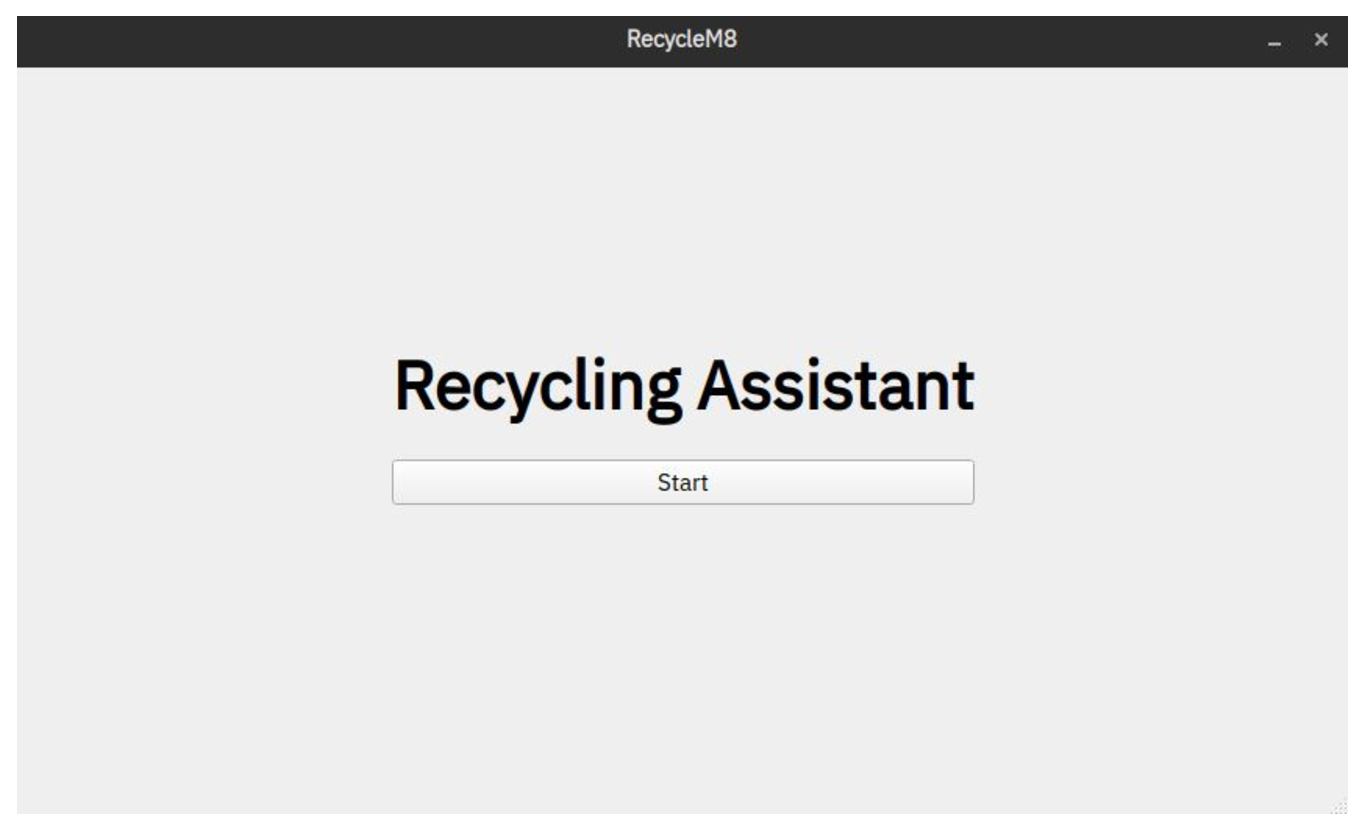
\includegraphics[width=0.48\textwidth]{images/start.eps}
    \caption{Initial Starting Page}
\end{figure}~\\

Once the "Start" button is clicked, they will be brought to the next menu. However, if the config file is valid (ie. does not fail the checks outlined in specification C: Reading the Configuration File), and the "skip\_start" settings flag is enabled, the application will skip directly to the scanning window, skipping the appearance of specification A: Initial Page.~\\

\subsection{Config File}
Upon application start, the settings/config file will be read. The settings/config file will read for and expect the following JSON values:~\\

\begin{itemize}
\item source\_type: int
\item source\_index: int
\item source\_str: string
\item skip\_start: bool
\item dashboard\_link: string
\item db\_enabled: bool
\item db\_conn\_str: string
\end{itemize}~\\

The application will perform a rudimentary valuation check. Since source\_type or source\_index are values that cannot be negative, if it detects this, then it will throw an invalid config error, and redirect the user to regenerate a new base config. This will then be loaded in memory in for internal reference within the application.

Whenever settings are changed, the config file should reflect those changes, also keeping a backup version of the config file as a contingency. As a result, if the settings are corrupted, the user may be able to recover their older settings from the backup file.~\\

\subsection{Reading the Configuration File}
The settings/config file will be stored in the directory under the name "settings.json", in the JSON format. The conditions that would cause an error are the following:~\\

\begin{quote}
\subsubsection{File Not Found}~\\
If the configuration file is not in the directory, or if it has not been generated yet (ie. user's first launch).
\end{quote}

\begin{quote}
\subsubsection{JSON Initial Document Parse Failure}~\\
If the JSON parser encounters an issue while reading the file due to it being in an invalid JSON format, or corrupted.
\end{quote}

\begin{quote}
\subsubsection{JSON Validity Failure}~\\
If the JSON file is empty (typically resulting from unexpected closing/crashing while writing to the file).
\end{quote}

\begin{quote}
\subsubsection{JSON Objects Failure}~\\
If the JSON does not contain the required objects, or has an unexpectedly incorrect type.
\end{quote}

\begin{quote}
\subsubsection{JSON Value Failure}~\\
If the JSON does not contain valid values in its objects. The validation process of the JSON Values will be explained in a later specification.
\end{quote}~\\

In the case of an error, the user will be directed to the Settings Not Found menu, in specification C: Settings Not Found, so that they have the option to regenerate a new config file.~\\

\subsection{Settings Not Found}
If the application does not detect the settings/config file, or if it is either corrupted or unreadable (more details in specification C: Reading the Configuration File), the user will be notified that the application will launch with default parameters, while also being notified that it will generate a new Config file. This means that any existing file will be overwritten and regenerated with default values.~\\

If the user accepts (OK button), the application will proceed with the creation of a new Config file, while the user may also reject (Cancel button) to return to the previous screen, so that they may either try to manually adjust the JSON file, or save the parameter values before the file is overwritten.~\\

Then, the user will be directed to the detection/scanner screen, if they chose to generate a new config. 

\begin{figure}[!h]
    \centering
    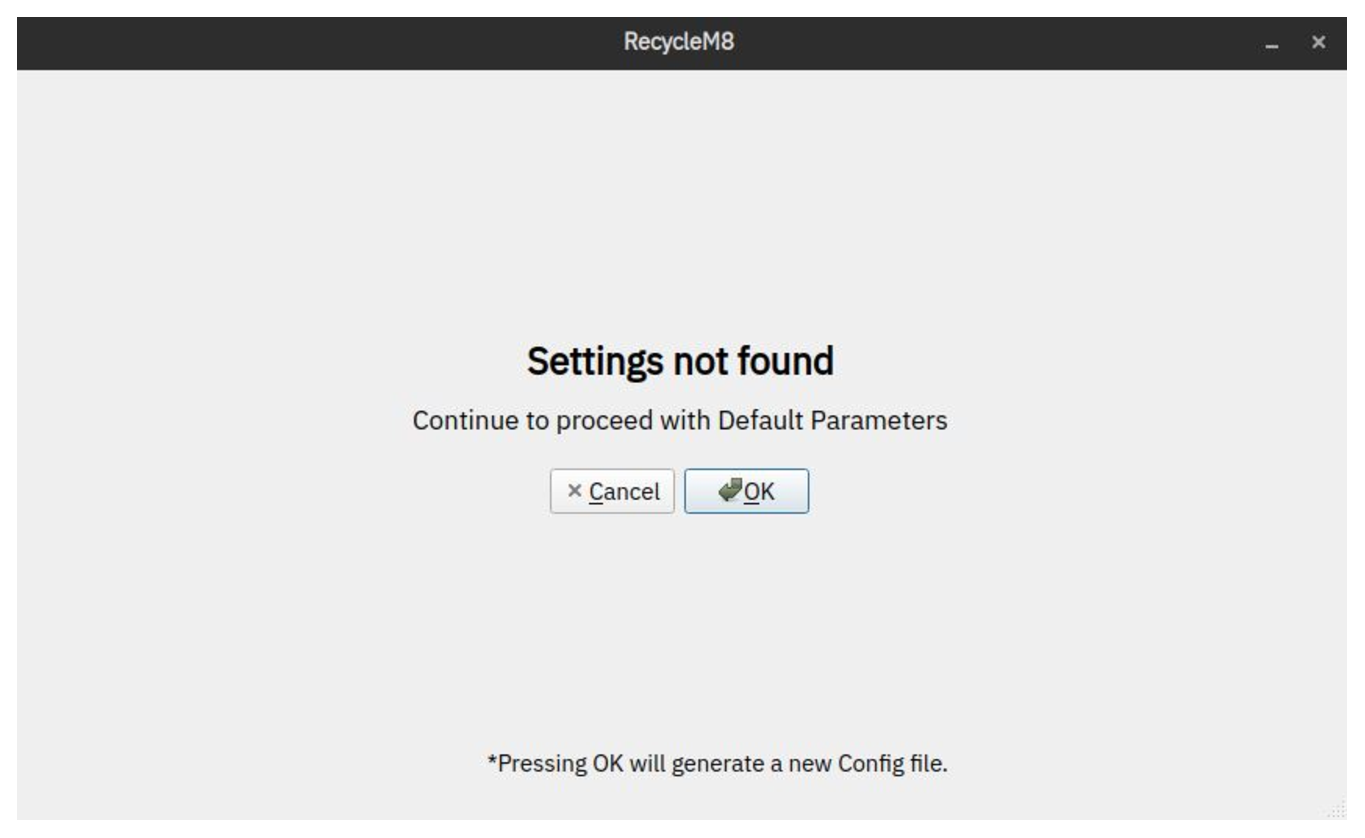
\includegraphics[width=0.48\textwidth]{images/settings_alert.eps}
    \caption{Settings Not Found Screen}
\end{figure}

\begin{figure}[!h]
    \centering
    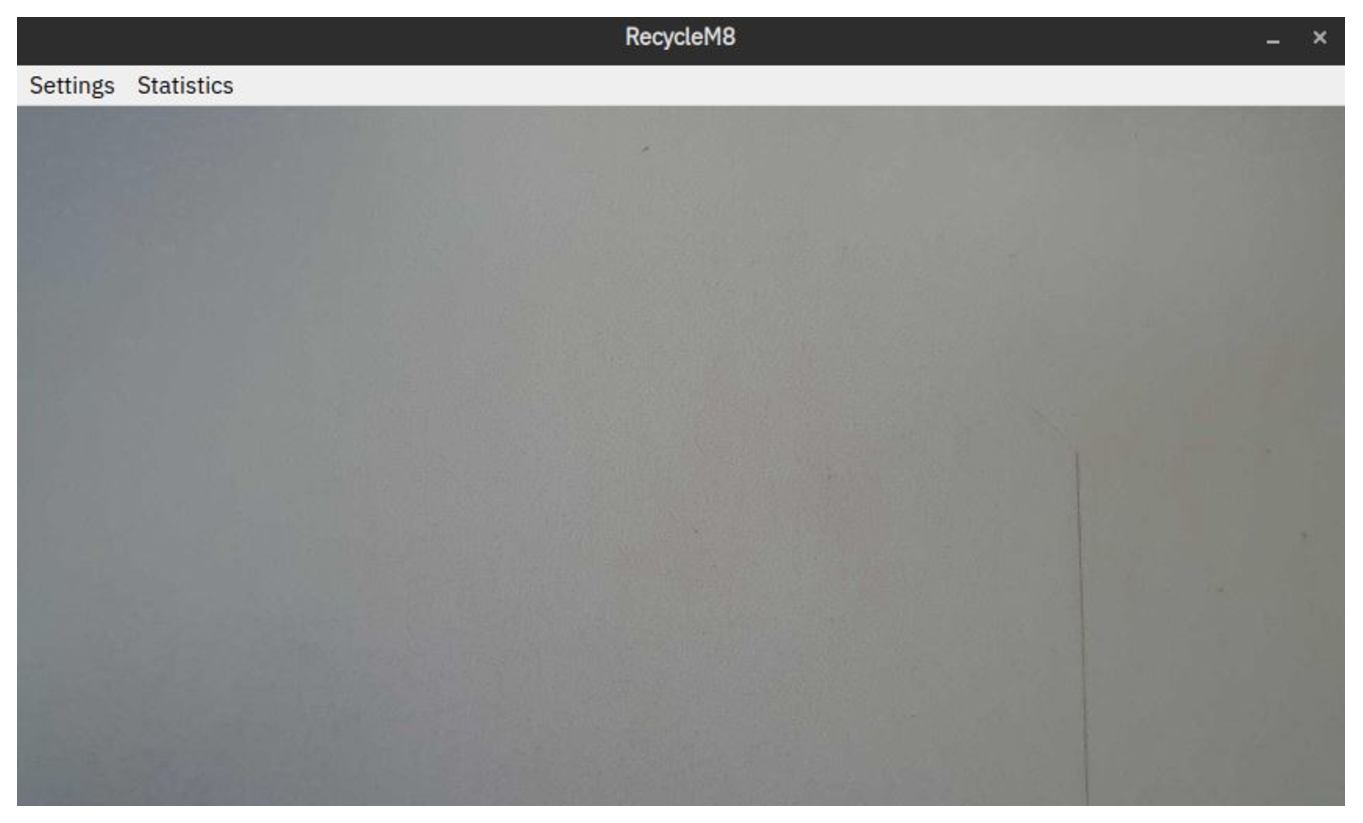
\includegraphics[width=0.48\textwidth]{images/nothing_detected.eps}
    \caption{User Proceeds with Generation of new Config (Presses OK), Proceeding to Scanner Screen}
\end{figure}

\begin{figure}[!h]
    \centering
    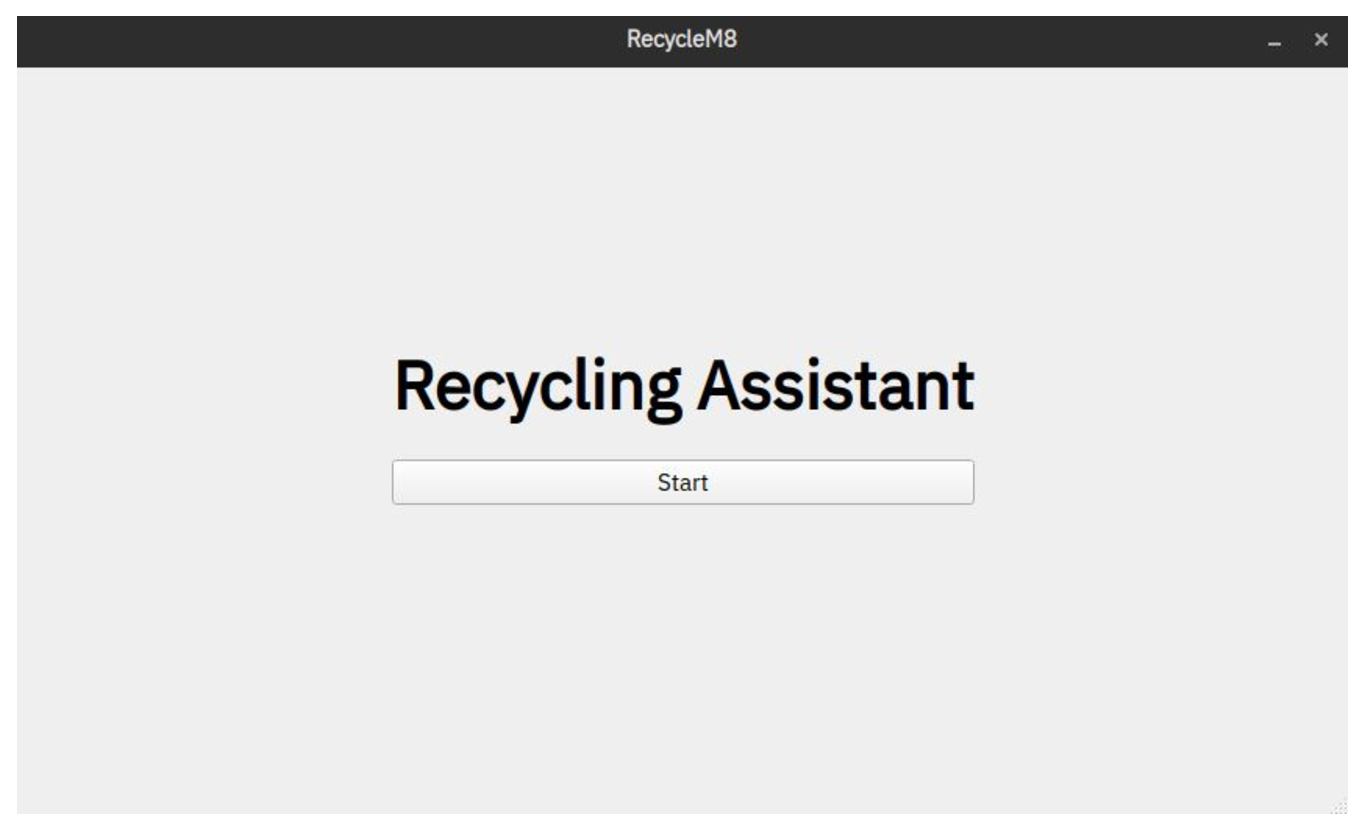
\includegraphics[width=0.48\textwidth]{images/start.eps}
    \caption{User Denies Generation of new Config (Presses Cancel), Reverting to Start Screen}
\end{figure}~\\

\newpage
\subsection{Failure to Connect to the Camera}
In the event that the application was not able to connect to the camera (usually occurring if the camera is not connected or offline), the user will be notified with a message box stating that there was an issue connecting to the camera. This message box will be modal, and prevent the user from interacting from the background window - they must agree or close the message box to re-assume control of the main window.~\\

They will see an empty detection screen, but will be able to access the settings menu in the top left corner (status bar). This will allow the user to adjust their set source, change other settings, and reset their connection, to try and re-establish a connection to the camera.~\\

\begin{figure}[h]
    \centering
    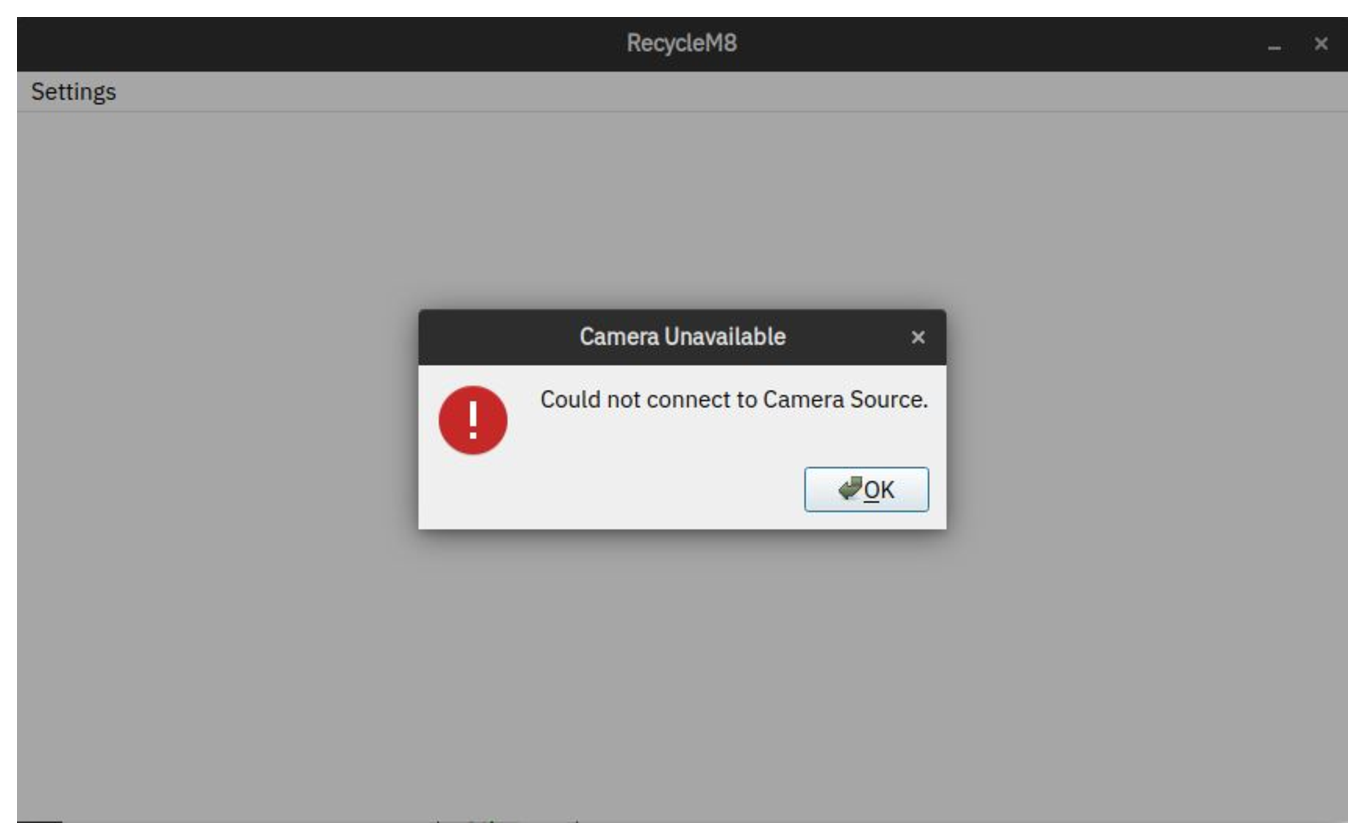
\includegraphics[width=0.48\textwidth]{images/camera_source_error.eps}
    \caption{Dialog Window Notification, Modal - Disables Main Window, but Keeps it Visible in the Background}
\end{figure}

\begin{figure}[h]
    \centering
    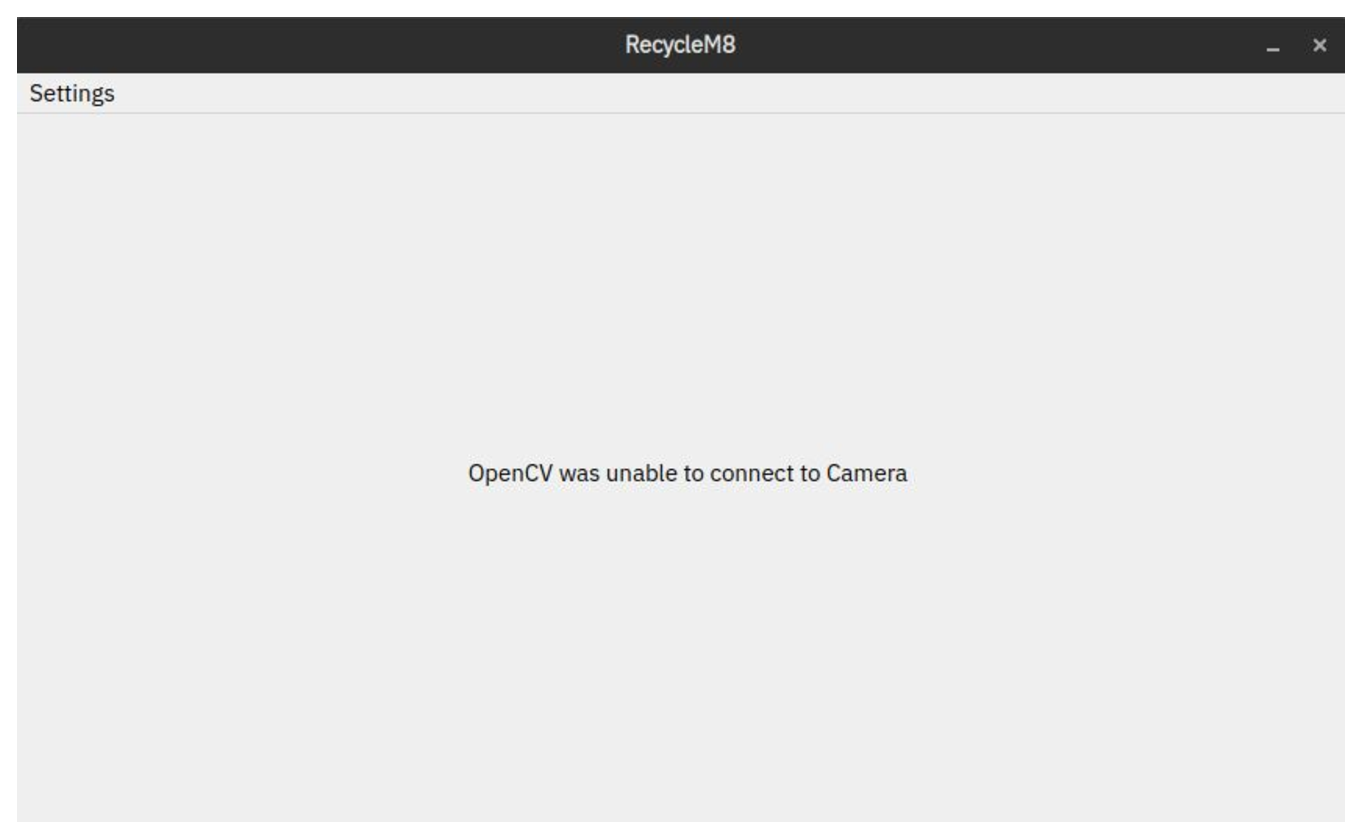
\includegraphics[width=0.48\textwidth]{images/camera_source_error_2.eps}
    \caption{After Dismissing Dialog Window Notification}
\end{figure}

\begin{figure}[h]
    \centering
    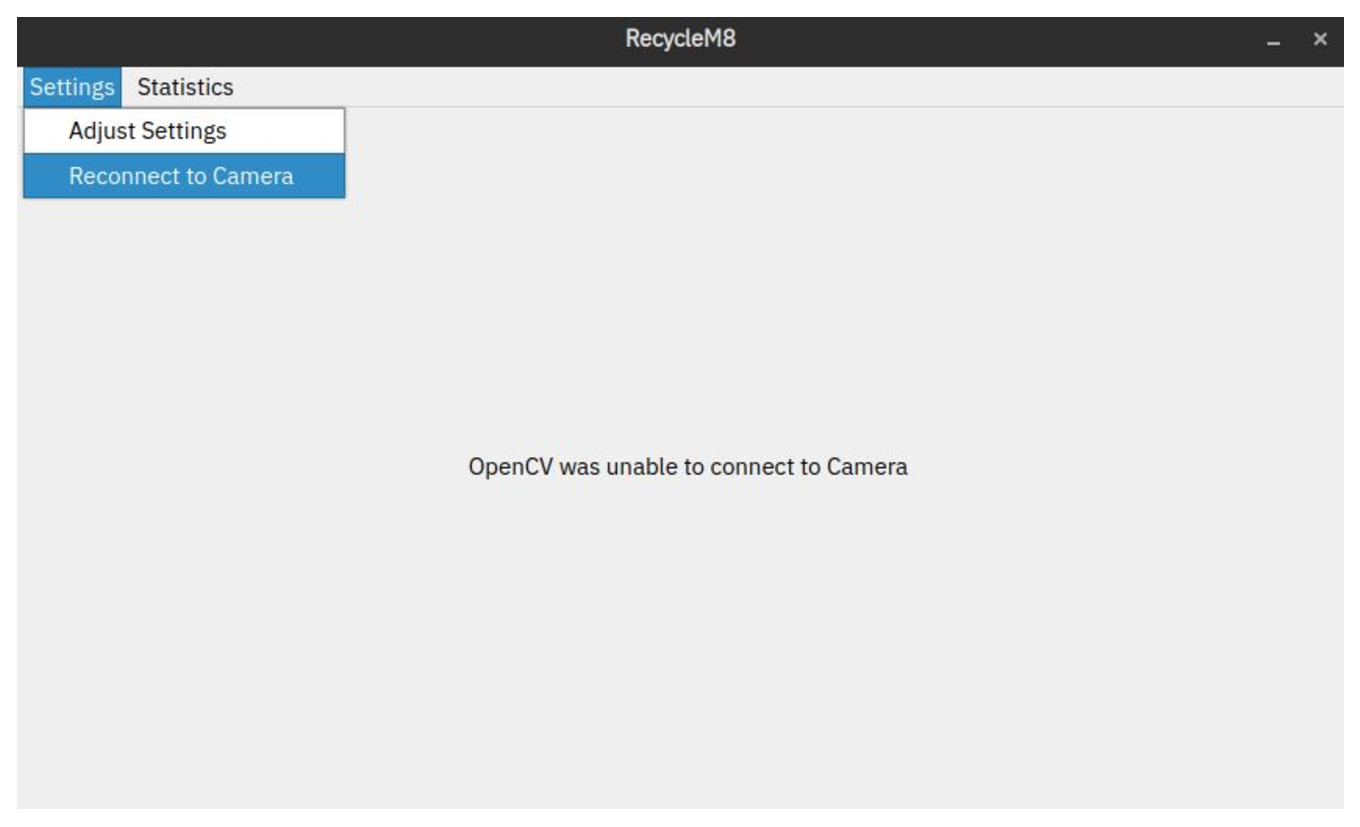
\includegraphics[width=0.48\textwidth]{images/reconnect_to_camera_context.eps}
    \caption{Reconnect Context Menu Action, allowing the user to restart or retry the Camera Connection}
\end{figure}

\begin{figure}[h]
    \centering
    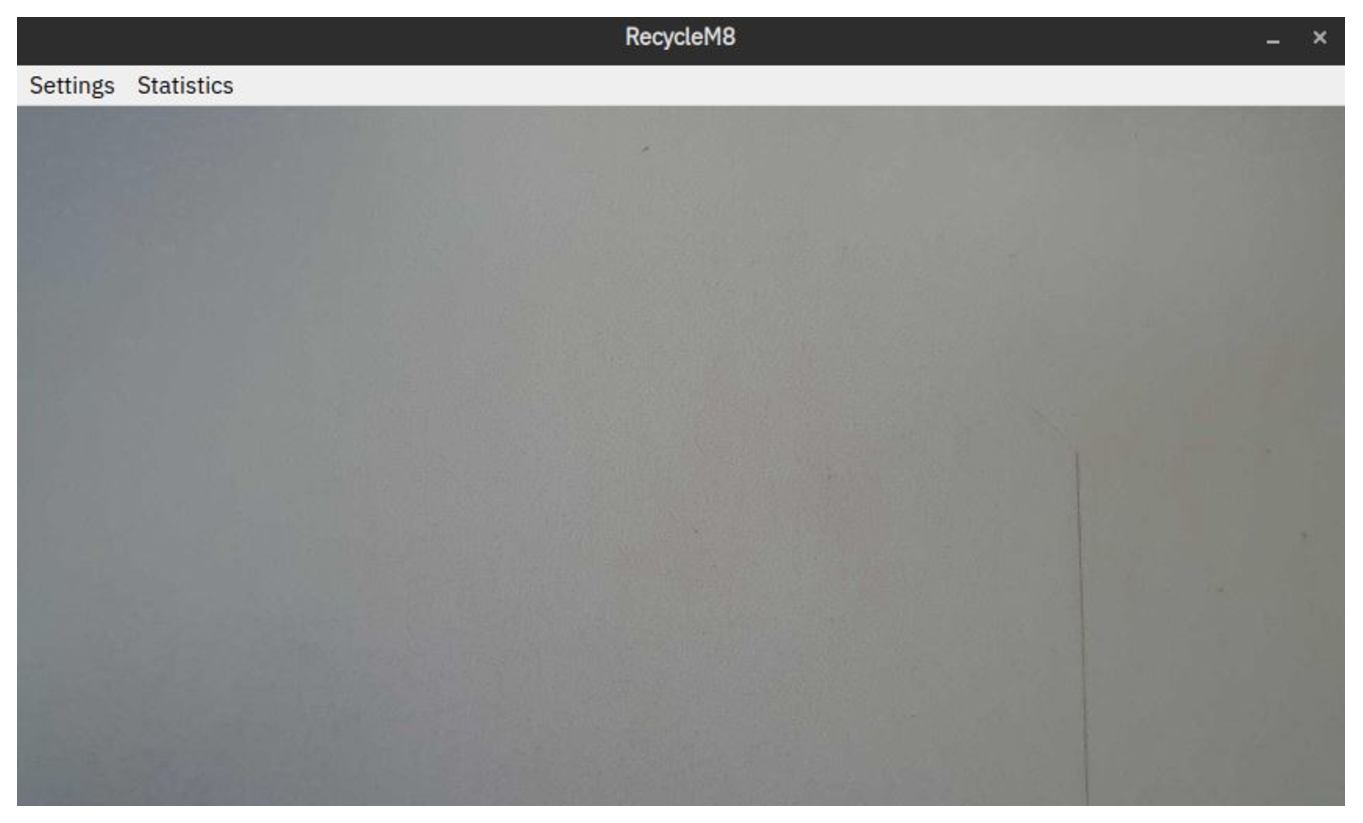
\includegraphics[width=0.48\textwidth]{images/nothing_detected.eps}
    \caption{Successful Reconnect (Normal Detection/Scanner Screen)}
\end{figure}

\begin{figure}[h]
    \centering
    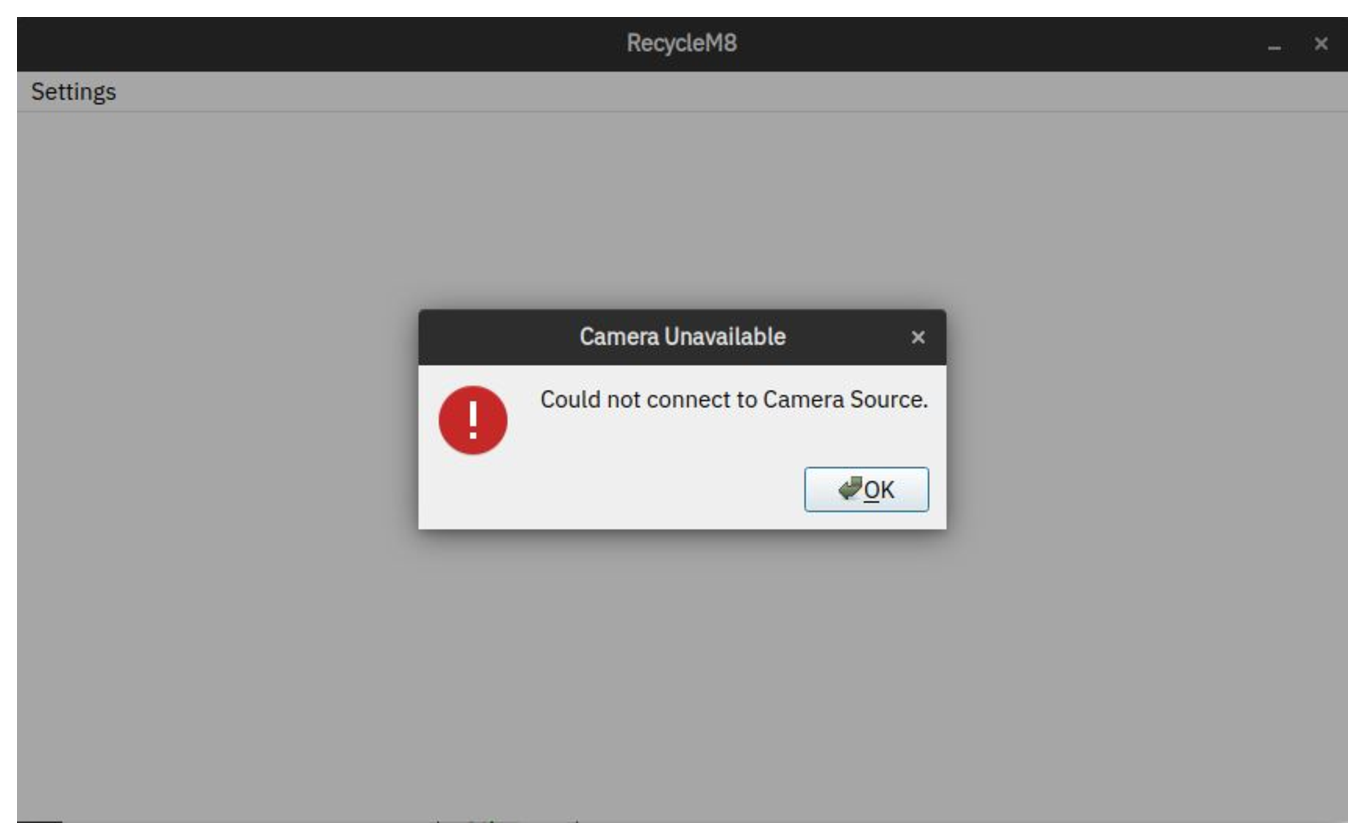
\includegraphics[width=0.48\textwidth]{images/camera_source_error.eps}
    \caption{Unsuccessful Reconnect (Same Error Flow as Figure 5)}
\end{figure}~\\

\newpage
\subsection{Detection/Scanner Screen}
The detection/scanner element takes up the vast majority of the application window estate. In this screen, a live camera feed is shown, based on the connection value assigned to the camera.~\\

The default connection value is camera index 0 (the device index - 0 refers to the default camera for the system), however it can be assigned to another index, or to a video (ie. mp4 or webcam stream) through the settings menu. For a webcam stream, a valid webcam stream link must be provided.~\\

The image format should be correctly converted (from OpenCV's BGR output to RGB) for display in the application, and the webcam stream should not prevent or block the user from using any other user interface elements. In addition, the output frames will be appropriately resized to the window size in a 16:9 ratio.~\\

Unless something is detected, no bounding boxes or detection-related text will be shown. On successful detection however, bounding boxes and detection-related text will be shown.

\begin{figure}[!h]
    \centering
    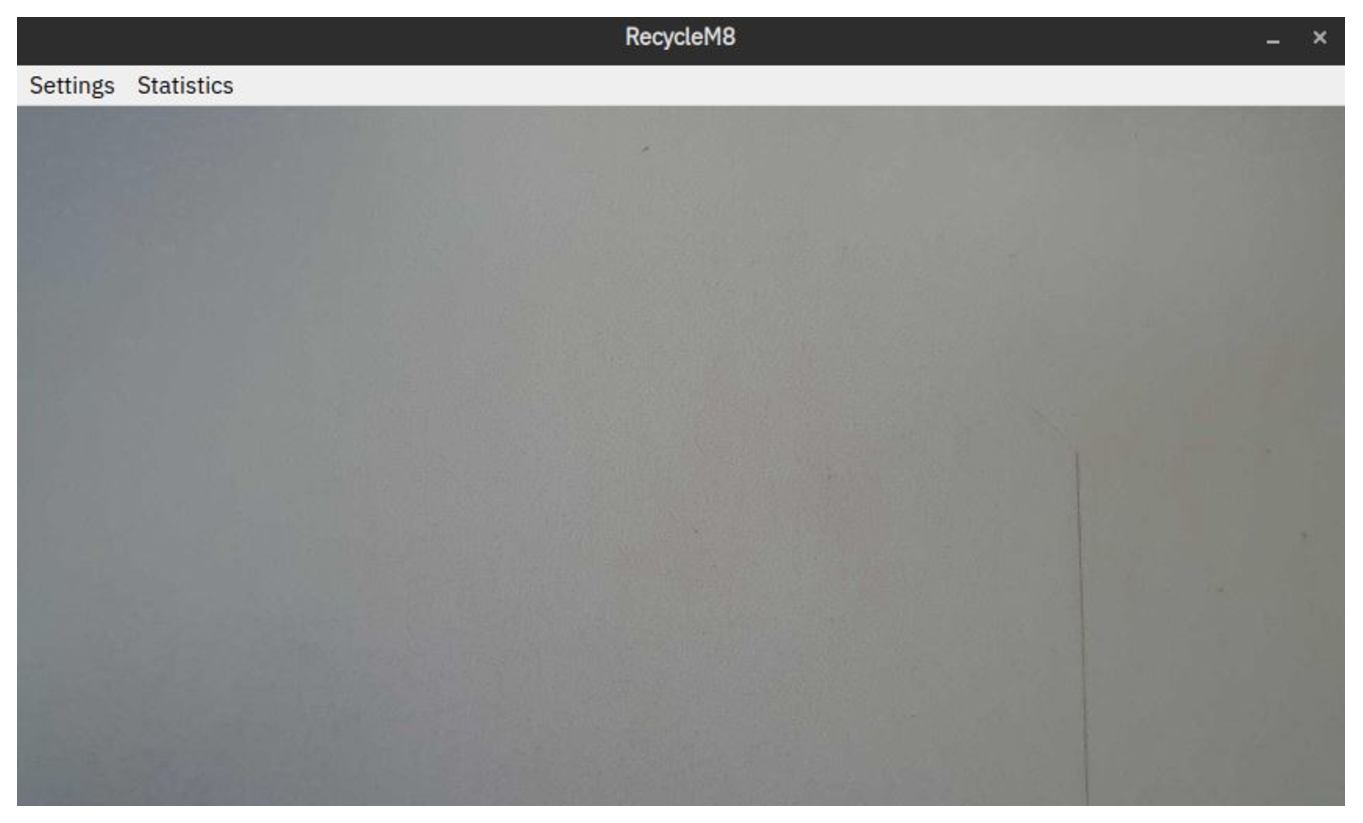
\includegraphics[width=0.48\textwidth]{images/nothing_detected.eps}
    \caption{Scanner Main Screen - Nothing Detected Yet}
\end{figure}

\begin{figure}[!h]
    \centering
    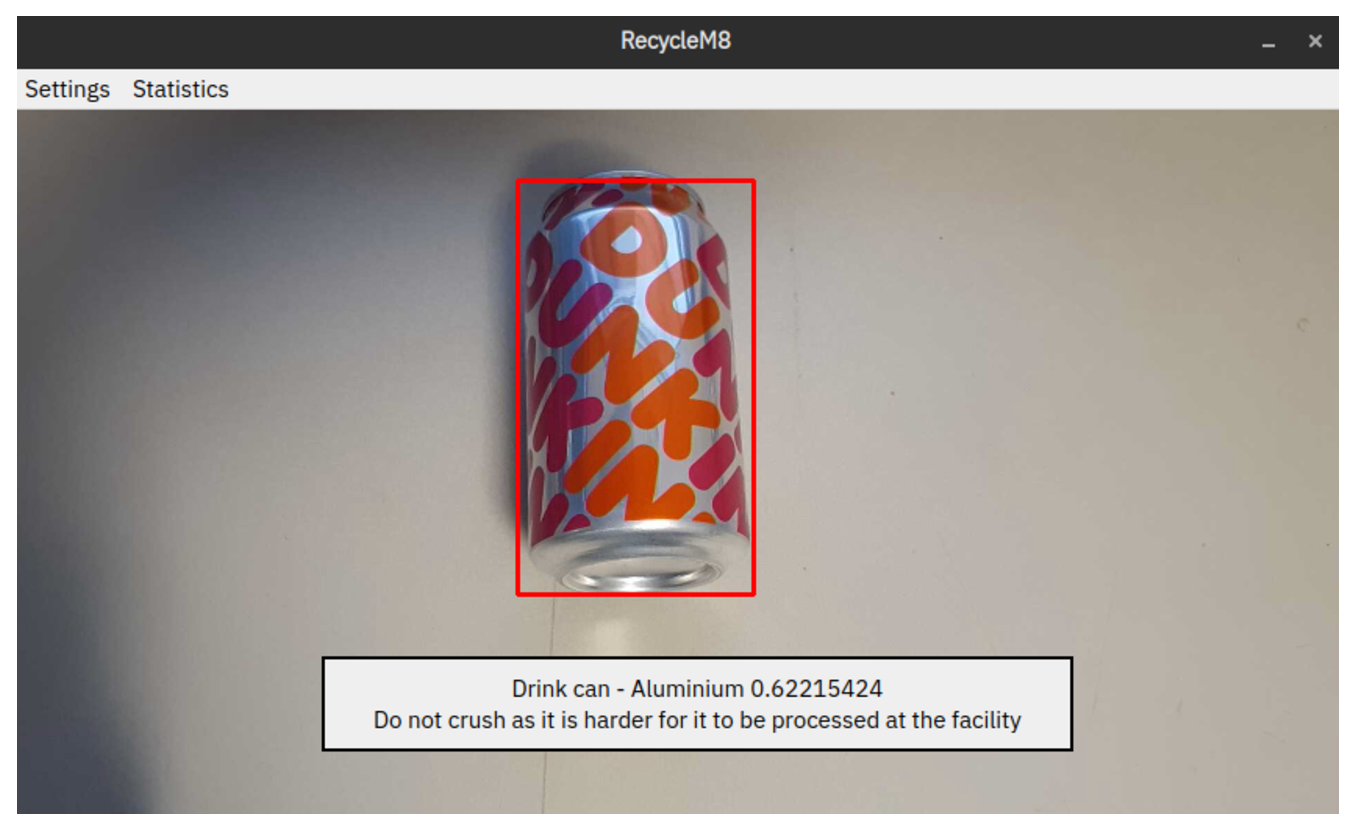
\includegraphics[width=0.48\textwidth]{images/successful_detection.eps}
    \caption{Scanner Main Screen - Object Detected}
\end{figure}~\\

\newpage
\subsection{Object Detection}
When an object is detected by the model, a bounding box will be drawn on the object, alongside what it recognized, and the confidence level. In addition, the recycling category and any special instructions will be displayed. Unknown objects or the background should not be detected.~\\

When an object class as a tip attached in the classification file, it will be shown alongside the detection in the text. For example, the tip to not pierce an aerosol canister, or not to crush an aluminum drink can. However, if the object does not have a tip attached, such as the metal bottle cap, then no tip will be shown - only the detected object name, and the recycling class (Metal).

\begin{figure}[!h]
    \centering
    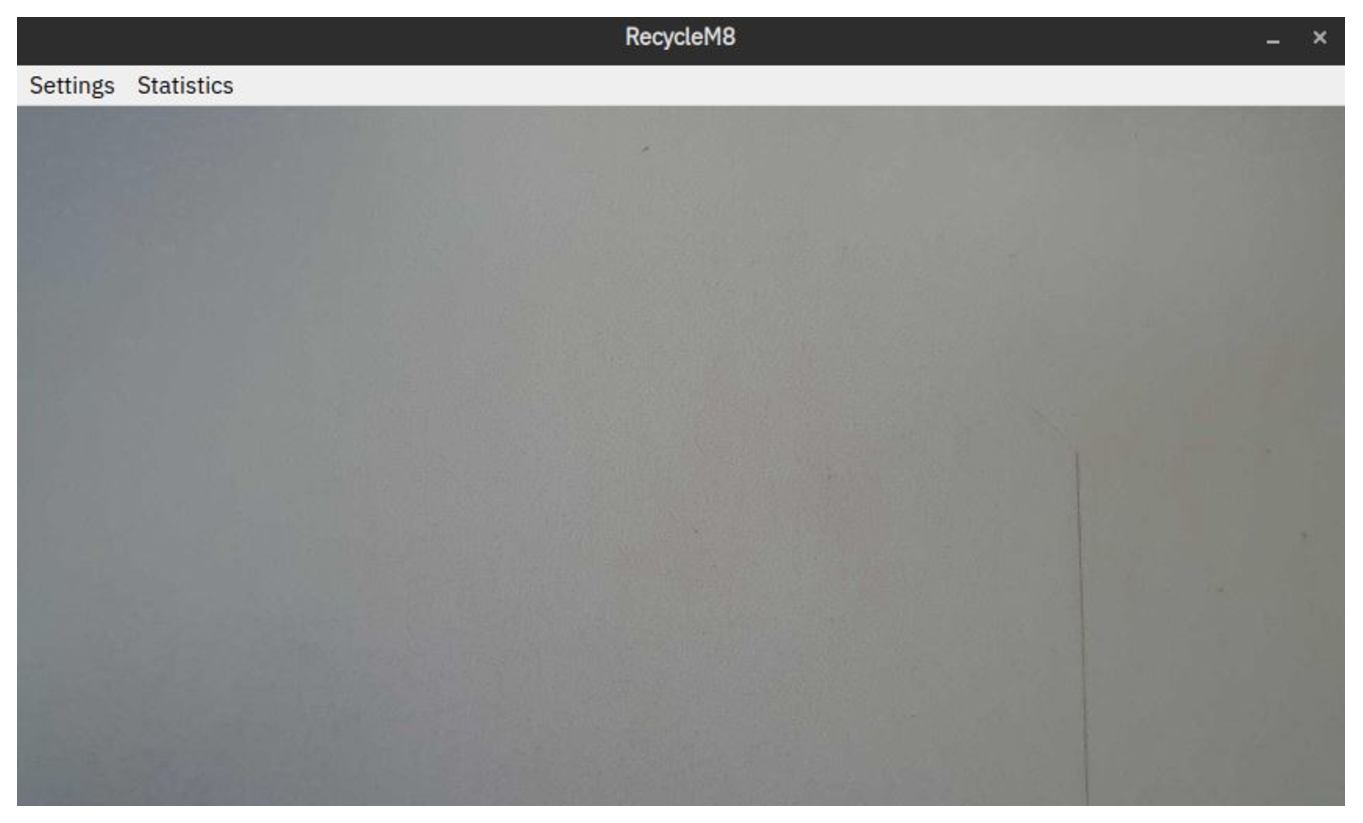
\includegraphics[width=0.48\textwidth]{images/nothing_detected.eps}
    \caption{Scanner Main Screen - Nothing Detected Yet}
\end{figure}

\begin{figure}[!h]
    \centering
    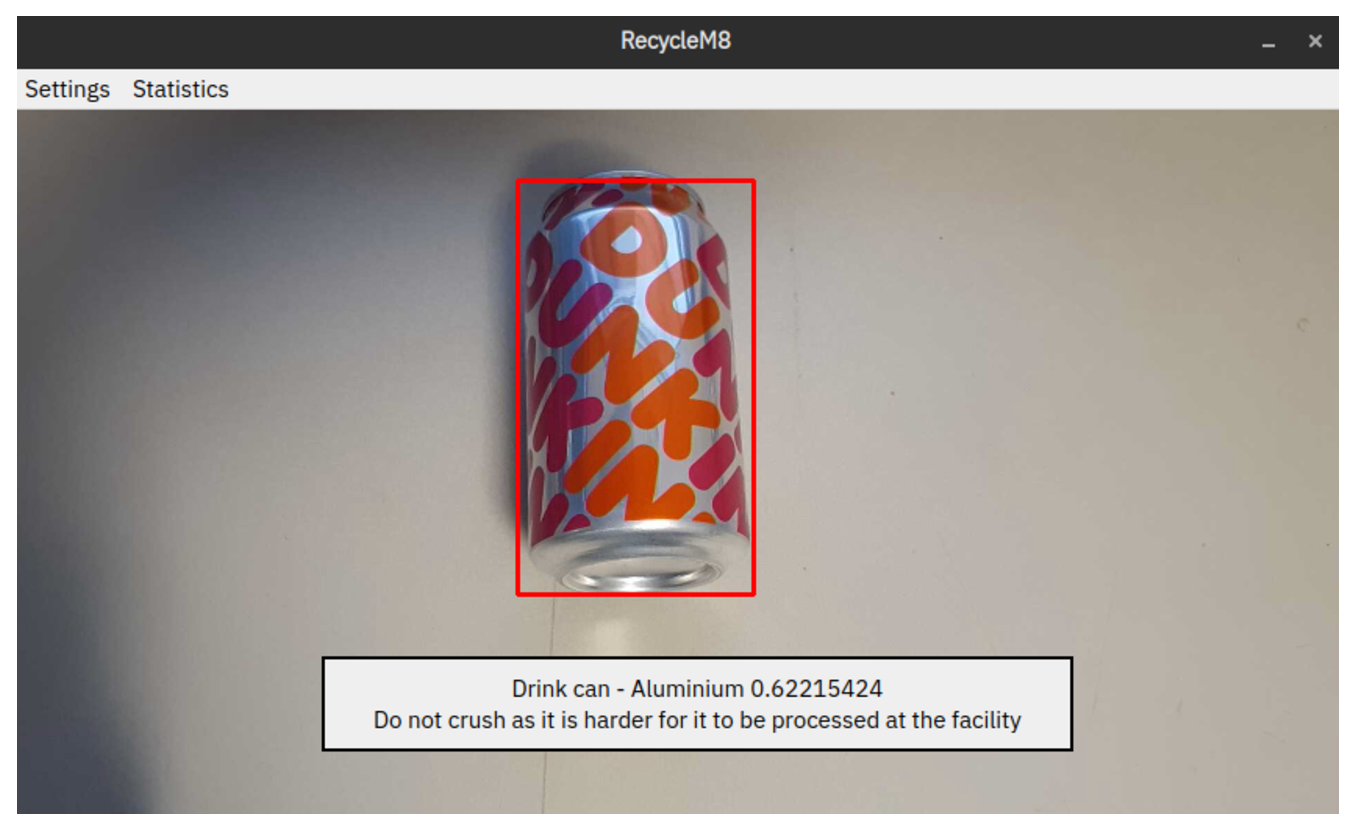
\includegraphics[width=0.48\textwidth]{images/successful_detection.eps}
    \caption{Scanner Main Screen - Object Detected, Tip Provided}
\end{figure}

\begin{figure}[!h]
    \centering
    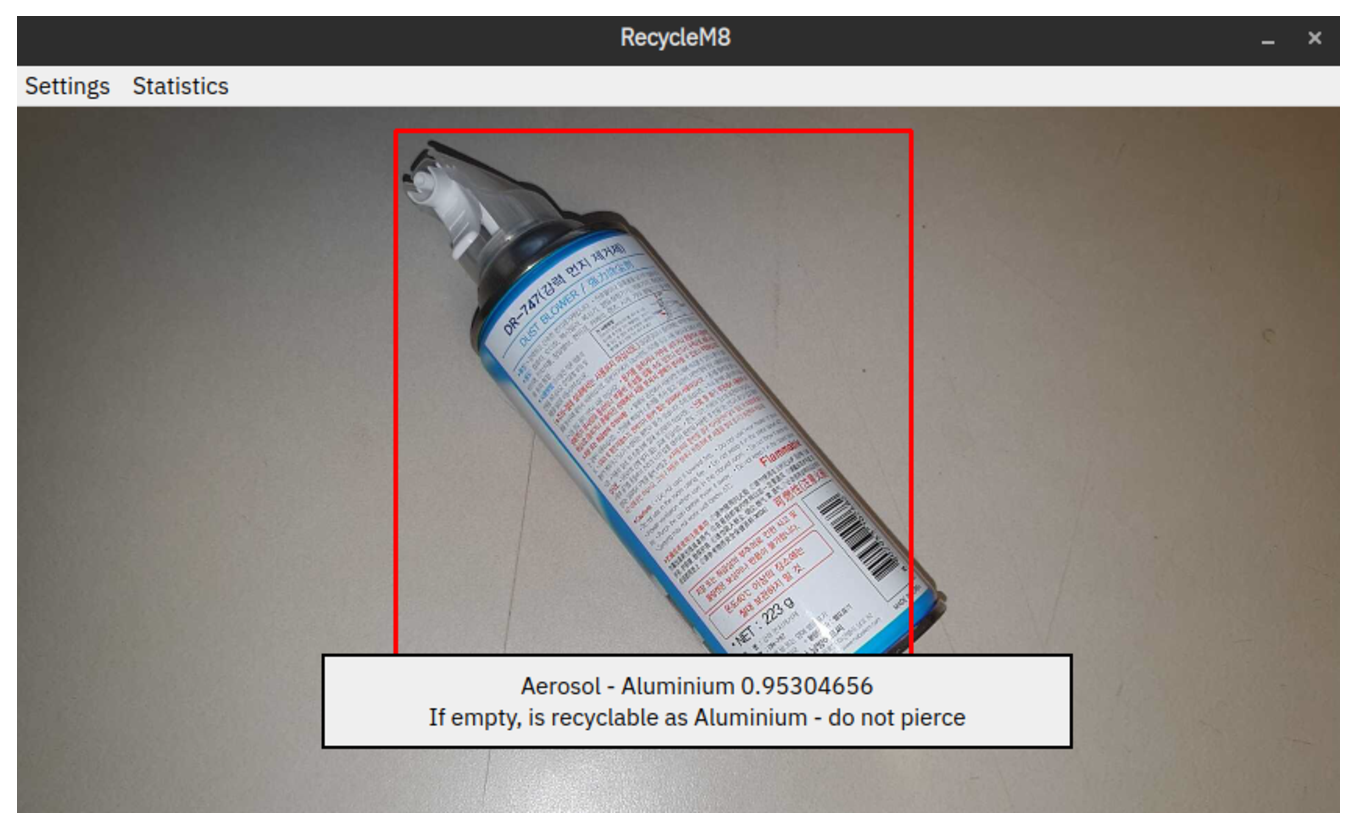
\includegraphics[width=0.48\textwidth]{images/aerosol_detected.eps}
    \caption{Scanner Main Screen - Object Detected, Tip Provided}
\end{figure}

\begin{figure}[!h]
    \centering
    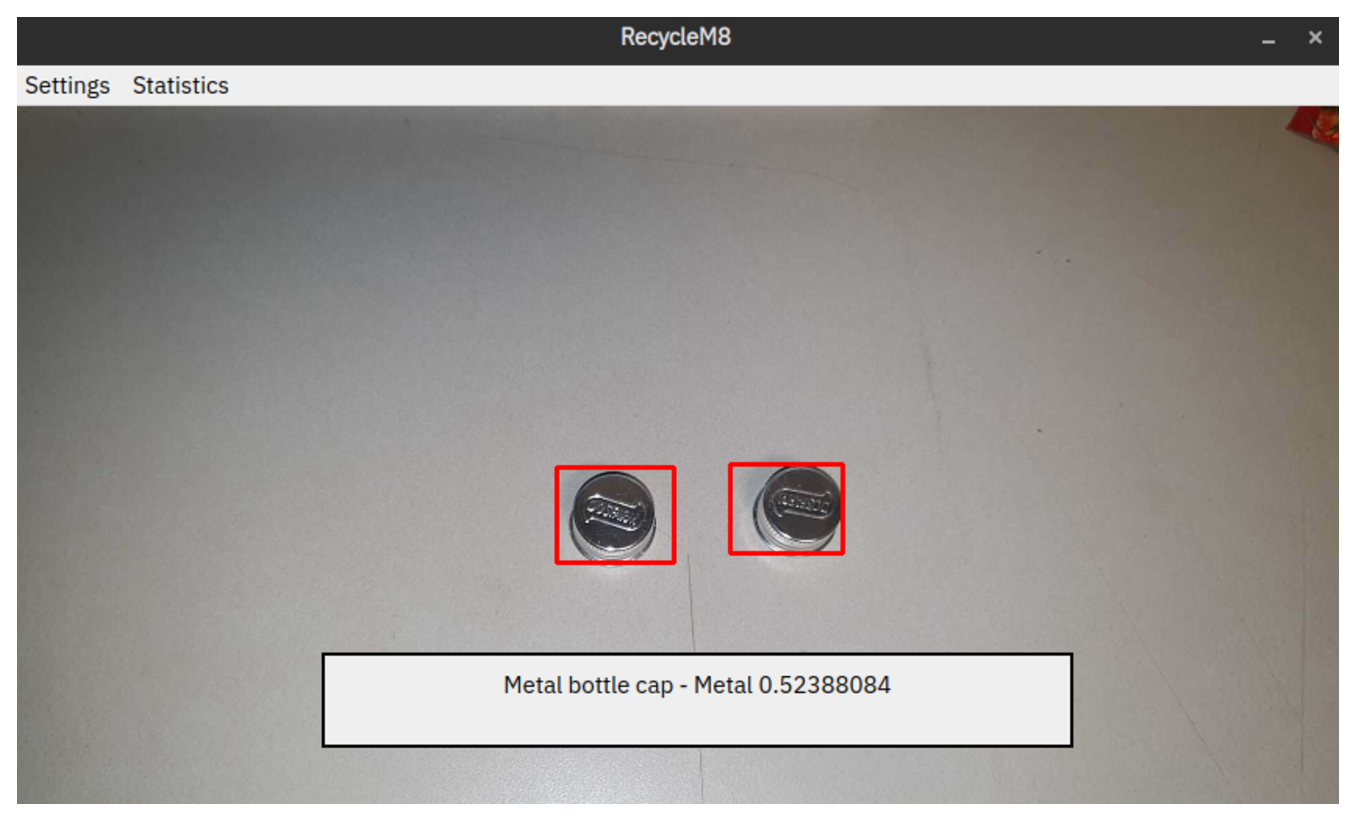
\includegraphics[width=0.48\textwidth]{images/bottlecap_detected.eps}
    \caption{Scanner Main Screen - Object Detected, No Tip to Provide}
\end{figure}~\\

\newpage
\subsection{Settings Menu}
When the user clicks on "Adjust Settings" in the Settings Context Menu Button, they will be presented with a modal Settings Menu Window. In the window, they will see three tabs - one for OpenCV Settings, one for Application Settings, and one for Database Settings.~\\

The Settings Menu's options should be synced with the actual config file values - the user's settings or the config file values should be represented in the Settings Menu, and any changes made in the Settings Menu should be immediately saved to the config file.~\\

\begin{figure}[!h]
    \centering
    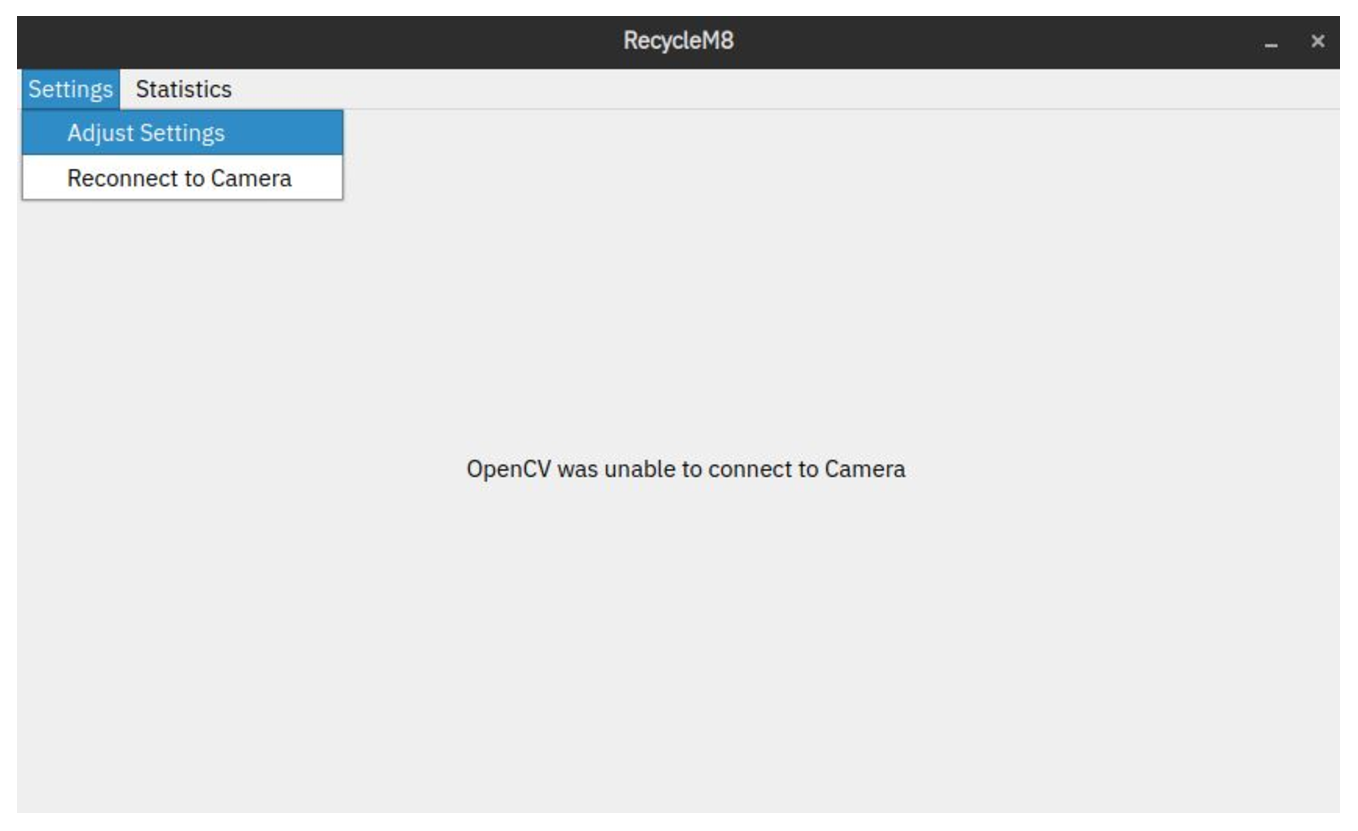
\includegraphics[width=0.48\textwidth]{images/adjust_settings.eps}
    \caption{Settings Context Menu Option}
\end{figure}~\\

\newpage
\subsubsection{OpenCV Settings}
This tab will contain settings related to OpenCV. The user will be able to choose between whether they would like to set their camera/stream based on the device index, or an IP address in the case of a webcam. The radio buttons will force the user to select one, and not both, but should not delete the saved value, allowing the user to store values - for easy switching between physically connected video sources, or web sources.~\\

\begin{figure}[h]
    \centering
    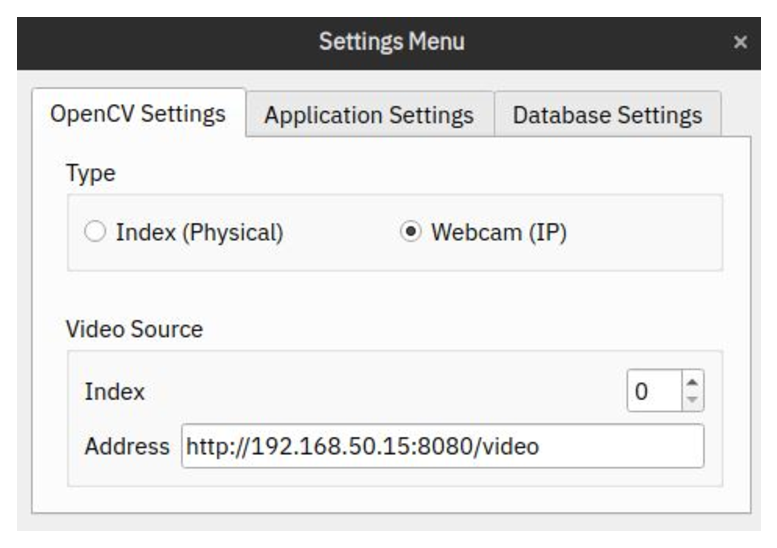
\includegraphics[width=0.48\textwidth]{images/opencv_settings.eps}
    \caption{OpenCV Settings Tab}
\end{figure}~\\

\subsection{Application Specific Settings}
This tab will contain settings related to the application. The user will be given the option to "Skip Start Sequence", which would make application starts skip directly to the detection screen. However, on startup, if the config file is deemed to be invalid, then the user will be sent to the "Settings Not Found" screen. 

As a result, on application startup, the config file will be checked for validity with priority, before checking the value of the "Skip Start Sequence" setting.~\\

\begin{figure}[h]
    \centering
    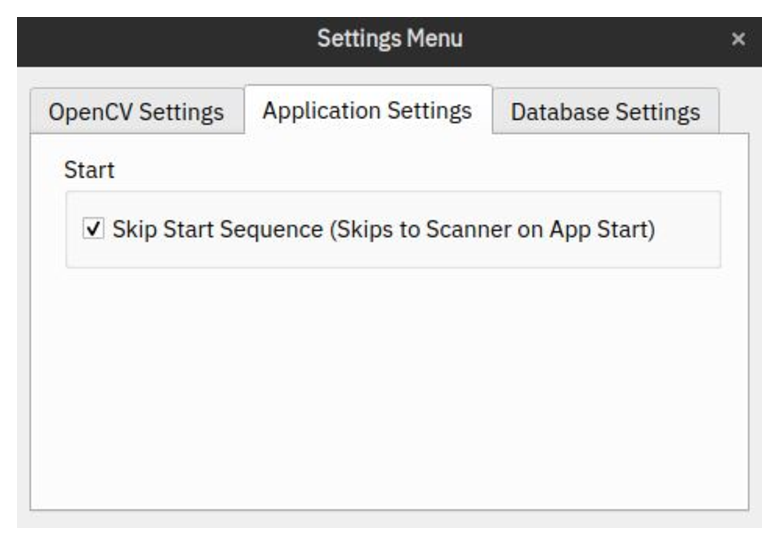
\includegraphics[width=0.48\textwidth]{images/app_settings.eps}
    \caption{Application Settings Tab}
\end{figure}~\\

\subsection{Classifications Handling}
A classifications file will read upon application startup. The classification file contains the following values:

\begin{itemize}
\item super\_categories: object (structure below)
\begin{itemize}
\item index: int
\item recyclable: bool
\end{itemize}
\item classifications: array (structure below)
\begin{itemize}
\item int (recycling category)
\item string (recycling tip)
\end{itemize}
\end{itemize}~\\

Upon startup, the classifications are loaded into an internal map to be referred to after inference. In addition, on database connection initiation (based on the db\_enabled setting), the existing database supercategory table is overwritten, and is loaded with the supercategory data from the classifications file.\\

\subsection{Database Settings}
This tab will contain settings related to the database. In this, the user may simply decide to choose to disable, or enable, the usage of database with regards to scans. The user may choose to do this if they would prefer not to have a database instance running, have no need for a database, or for privacy reasons or convenience reasons (ie. choosing not to run the dashboard).~\\

Specific settings such as the database connection string will only be accessible through direct editing of the config file, as the values are automatically set in relation to the separate setup stage for the database.~\\

\begin{figure}[h]
    \centering
    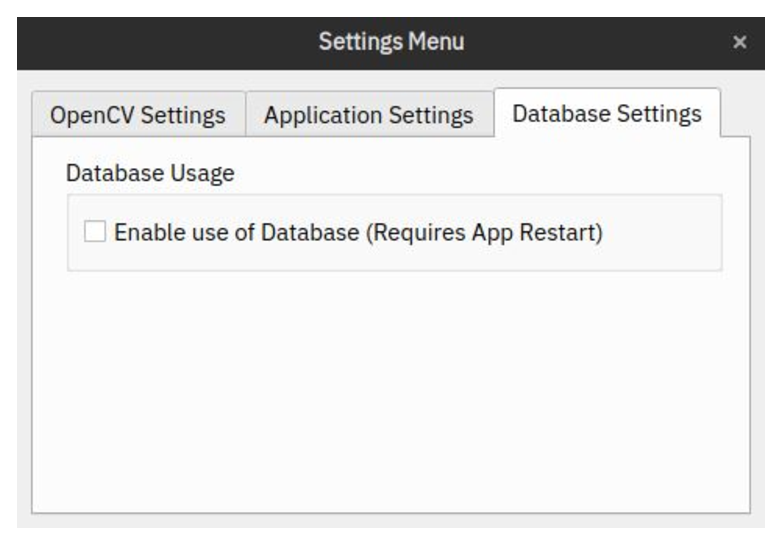
\includegraphics[width=0.48\textwidth]{images/db_settings.eps}
    \caption{Database Settings Tab}
\end{figure}~\\

\subsection{Statistics}
When the user clicks on "View Statistics" in the Statistics Context Menu Button, they will be presented with a Statistics Window. The window should be non-modal - as in, the user should still be able to interact with the other window at the same time while viewing statistics. In the window, they will see two tabs - one for session stats, and one for overall stats.~\\

\begin{figure}[h]
    \centering
    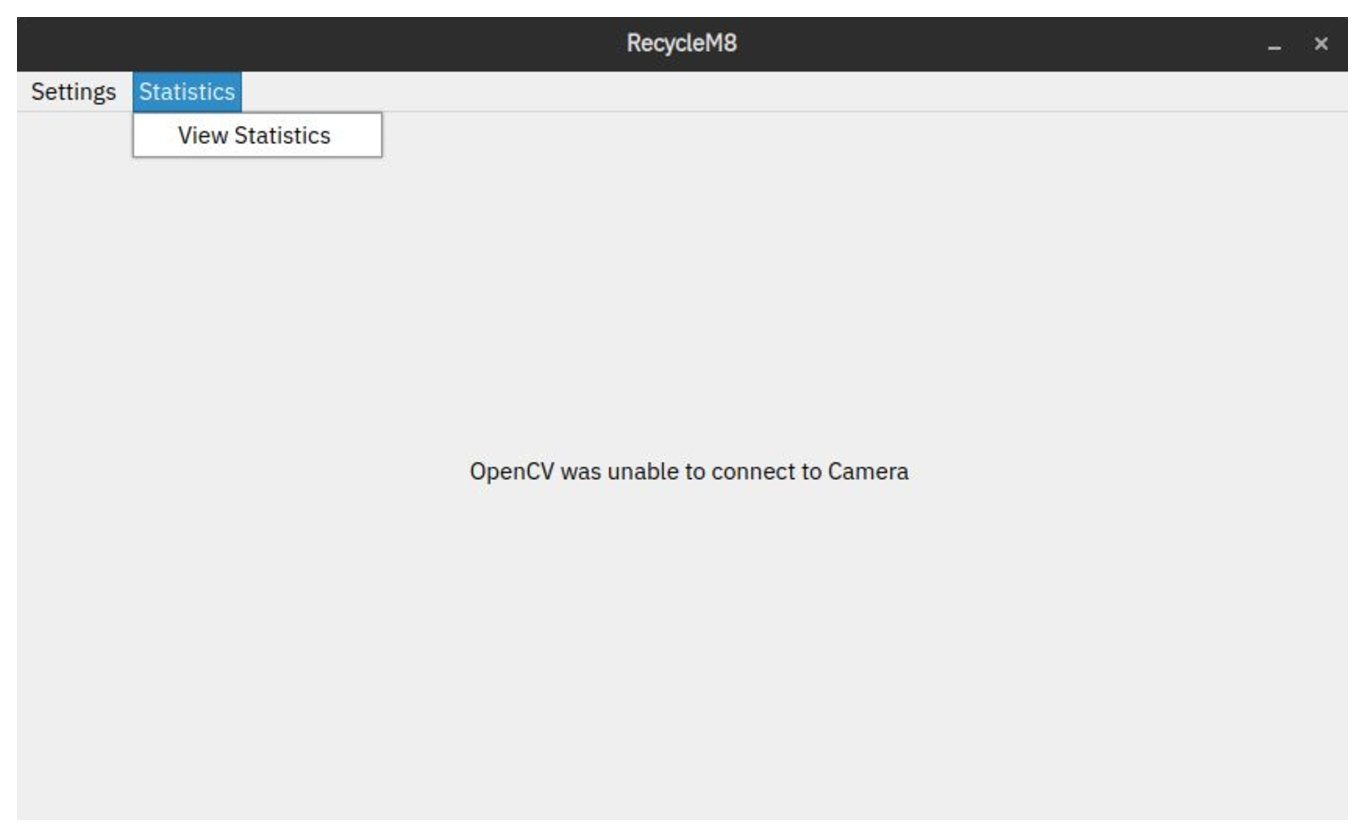
\includegraphics[width=0.48\textwidth]{images/stats_context_menu.eps}
    \caption{Statistics Context Menu}
\end{figure}~\\

\subsection{Session Statistics}
In the session stats window, they will see an "Overall Scan Count", and a "Categorical Scan Count". Overall scan count is self-explanatory - it is the number of times any object was scanned. Categorical scan count is the number of times an object from a category was scanned, divided by the overall scan count. The resulting percentage number is then rounded, and then fed into the progress bar. The categories will be divided into the following:~\\

\begin{itemize}
\item Plastic
\item Aluminium
\item Glass
\item Other
\end{itemize}~\\

\begin{figure}[h]
    \centering
    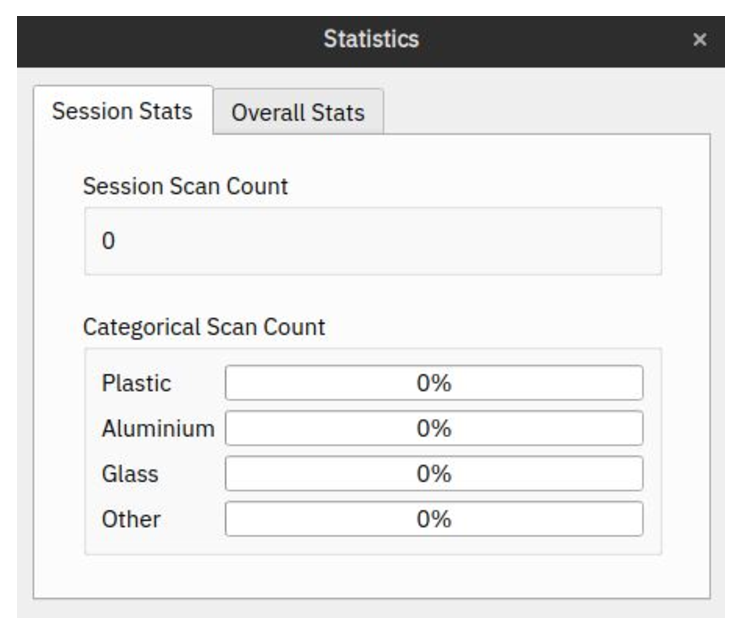
\includegraphics[width=0.48\textwidth]{images/empty_session_stats.eps}
    \caption{Unfilled Session Stats}
\end{figure}

\begin{figure}[h]
    \centering
    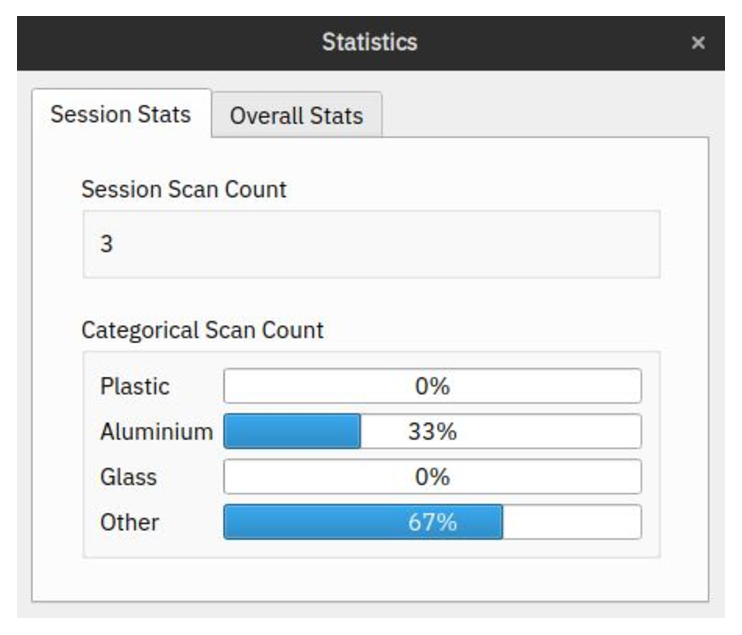
\includegraphics[width=0.48\textwidth]{images/filled_session_stats.eps}
    \caption{Filled Session Stats}
\end{figure}~\\

\newpage
\subsection{Overall Statistics}
This section is only functional if database is enabled and set up, as it requires database data in order to operate. It shows a button that will automatically launch the user's browser and direct them to the set dashboard for more in-depth information.~\\

\begin{figure}[h]
    \centering
    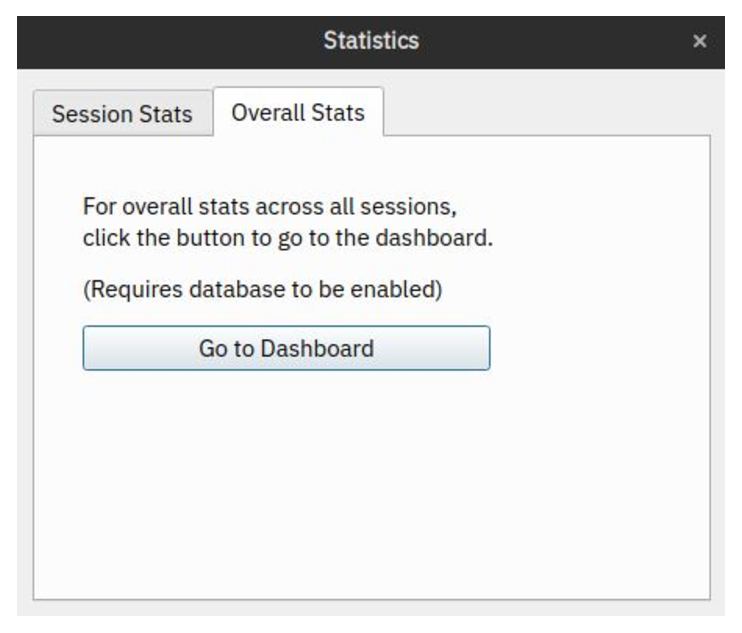
\includegraphics[width=0.48\textwidth]{images/stats_overall.eps}
    \caption{Overall Stats Tab}
\end{figure}~\\

\subsection{Exiting the Application}
The user may simply lick the top-right "x" button to close the application. However, as some of the windows or popup menus that appear may be modal (ie. Settings), the user will have to close those first before being able to close the application normally.~\\

\newpage
\subsection{Dashboard Charts}
In the dashboard window, it shows the number of detected objects for each hour and each super categories. The graph contains not all super categories, but displays top five most recognized super categories in a day.~\\

\begin{figure}[h]
    \centering
    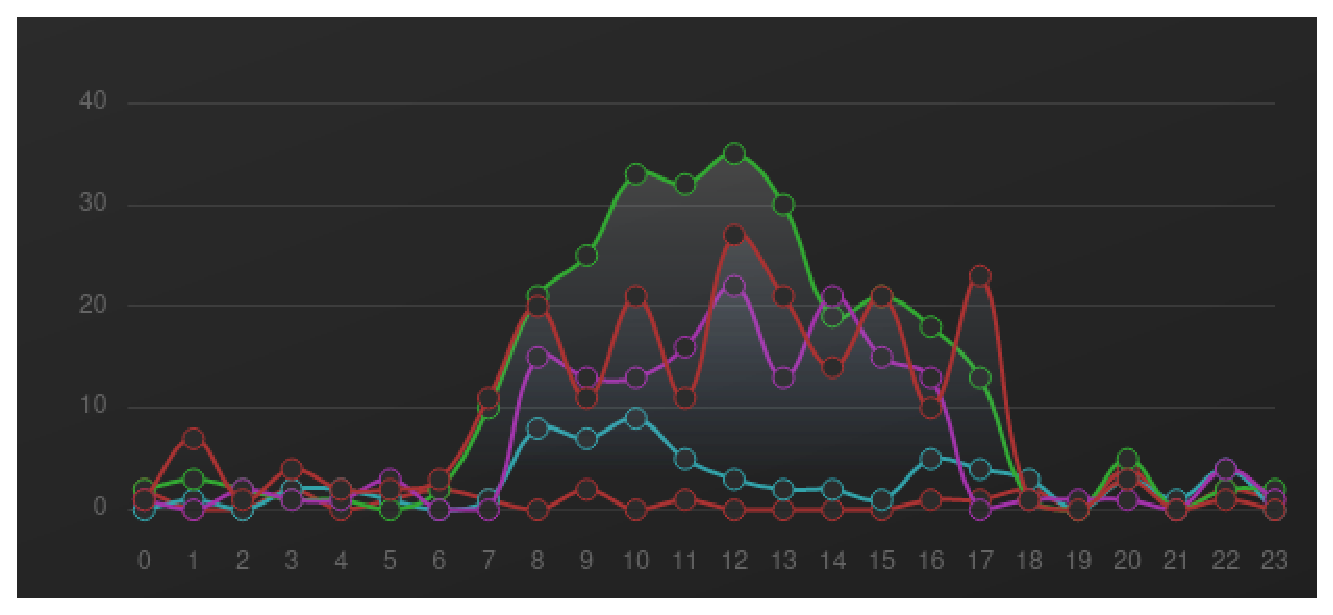
\includegraphics[width=0.48\textwidth]{images/chart_hourly_detected.eps}
    \caption{Hourly Detected Objects Chart}
\end{figure}~\\

Usage counts collects the overall number of detected images for a week. The images without any detection will be excluded in this statistics. It also contains today's records until the time of stats.~\\

\begin{figure}[h]
    \centering
    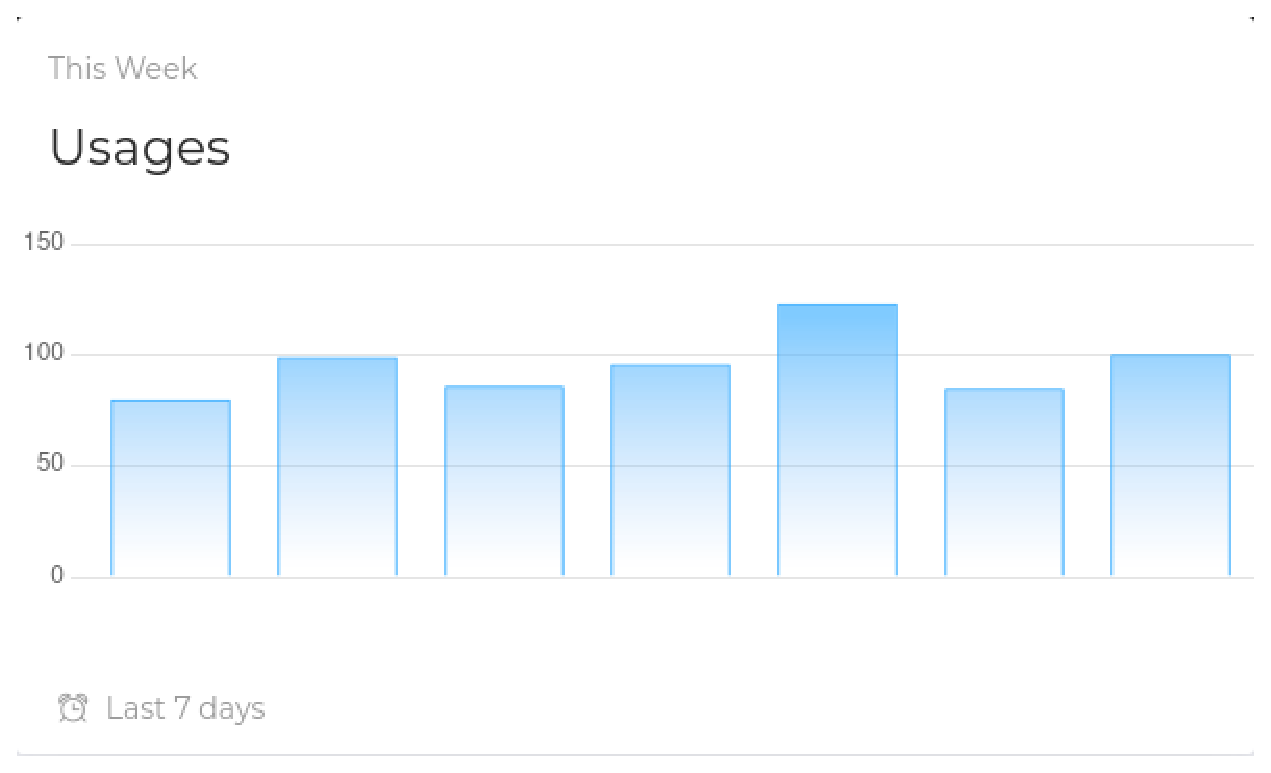
\includegraphics[width=0.48\textwidth]{images/chart_usage_counts.eps}
    \caption{Weekly Usages Chart}
\end{figure}~\\

Among the detected objects today, recyclable rates shows the percentage of recyclable objects for each hour. The number of objects which is marked as a recyclable ones is divided by the overall detection count. If an object has no label whether it is recyclable or not, those kinds of counts will be discarded in this statistics.~\\

\begin{figure}[h]
    \centering
    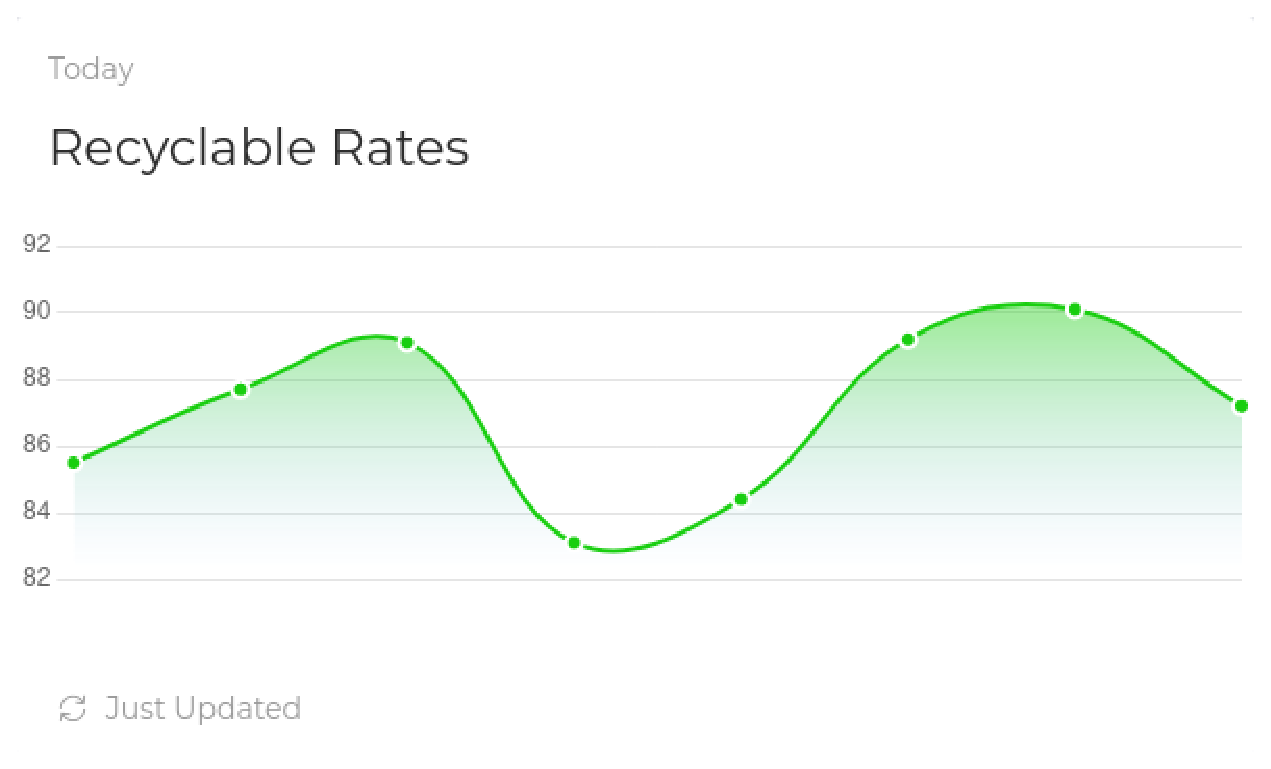
\includegraphics[width=0.48\textwidth]{images/chart_recyclable_rate.eps}
    \caption{Recyclable Rates Chart}
\end{figure}~\\

\newpage
Detection time chart tracks how long it takes to make an prediction for a scanned image in the precision of a millisecond. This statistics contains the average of these times for each hour of today. If there is no detection in some hours, the graph won't contain those hours in x axis.~\\

\begin{figure}[h]
    \centering
    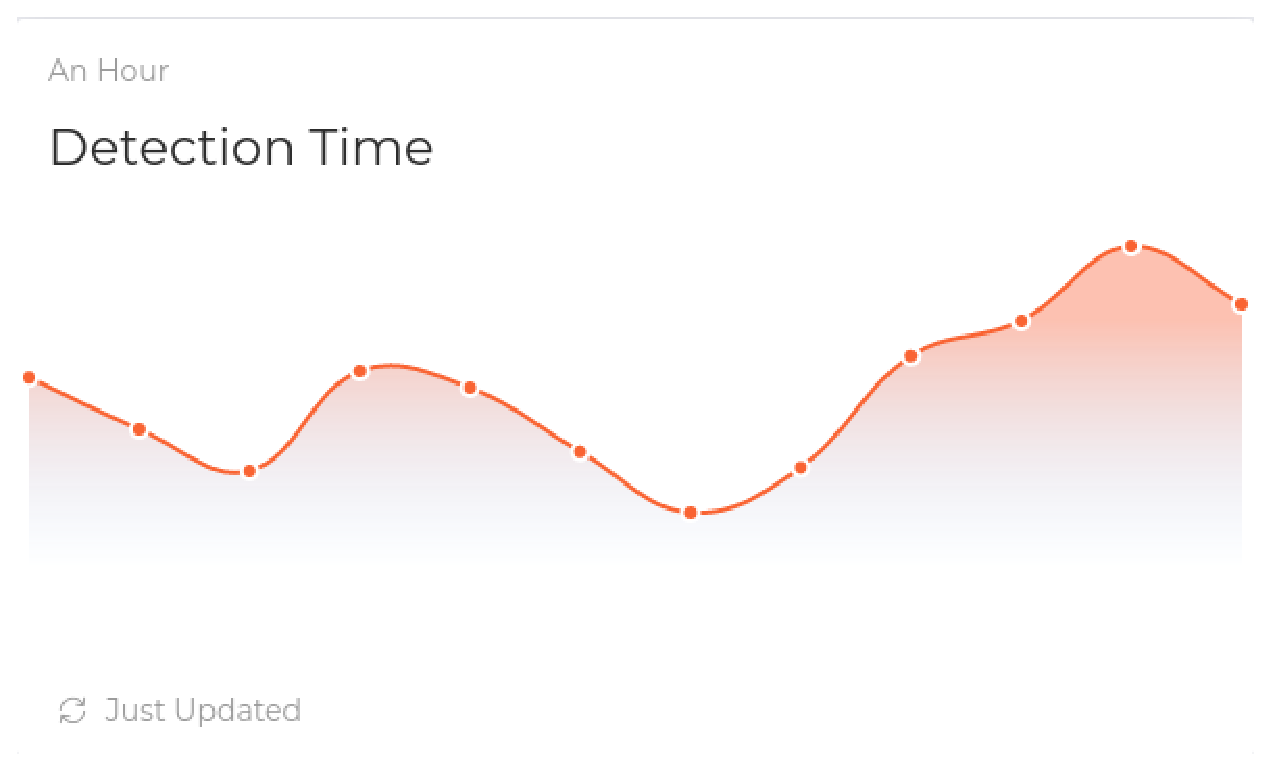
\includegraphics[width=0.48\textwidth]{images/chart_detection_time.eps}
    \caption{Detection Time Chart}
\end{figure}~\\

\newpage
\subsection{Dashboard Tables}
Monthly comparison table compares this month's scanned counts for each super category with the last month's one. This charts shows five super categories with the most counts at this month. The differences of numbers between two months will be also shown.~\\

\begin{figure}[h]
    \centering
    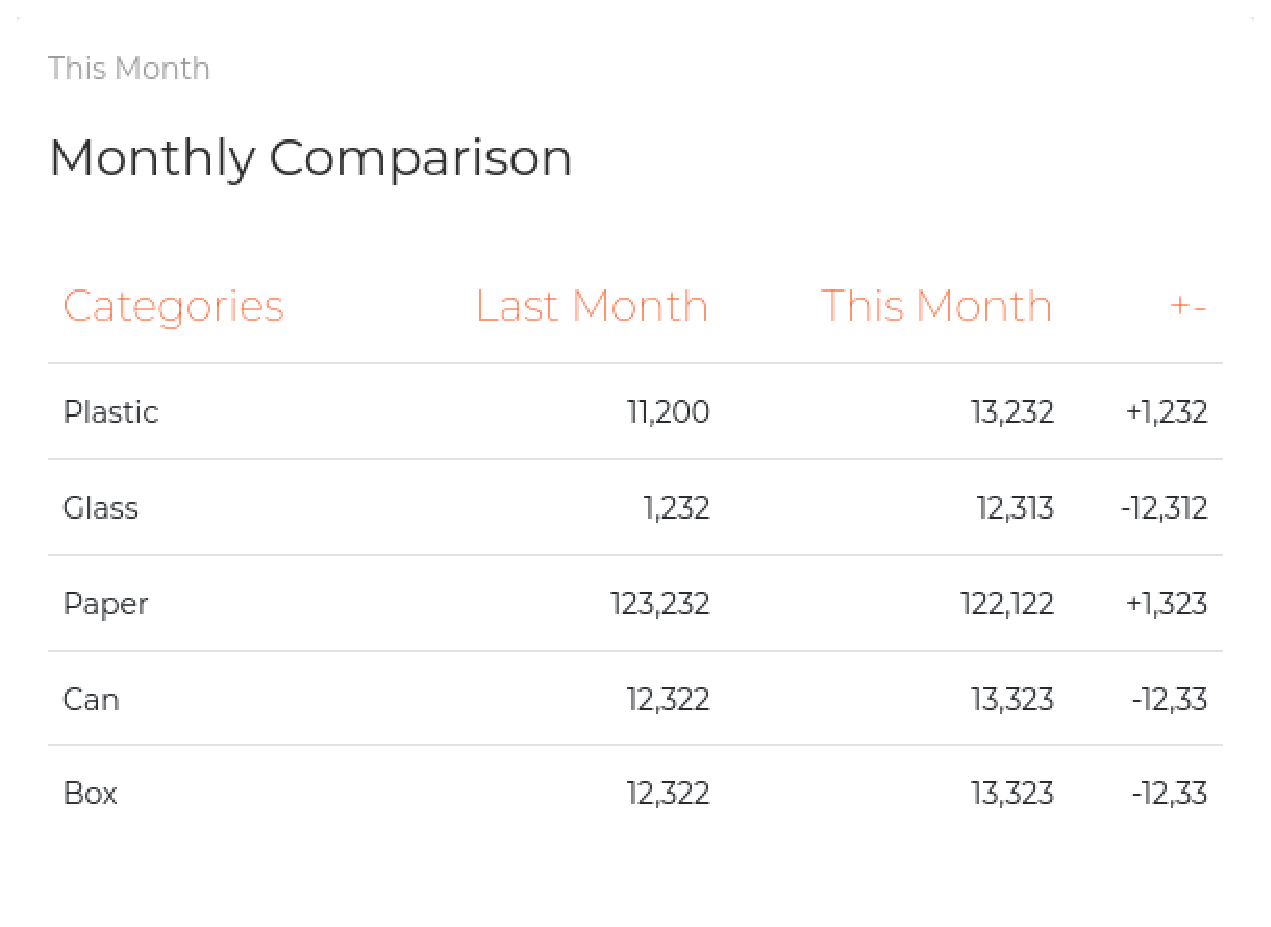
\includegraphics[width=0.48\textwidth]{images/chart_monthly_comp.eps}
    \caption{Monthly Comparisons Table}
\end{figure}~\\

Most detected objects table shows the cumulative counts of recyclable objects in this year. This list will have top 10 most detected objects' names with their super category. It also calculates the proportions of scanned objects, divided by the number of overall scanned images.~\\

\begin{figure}[h]
    \centering
    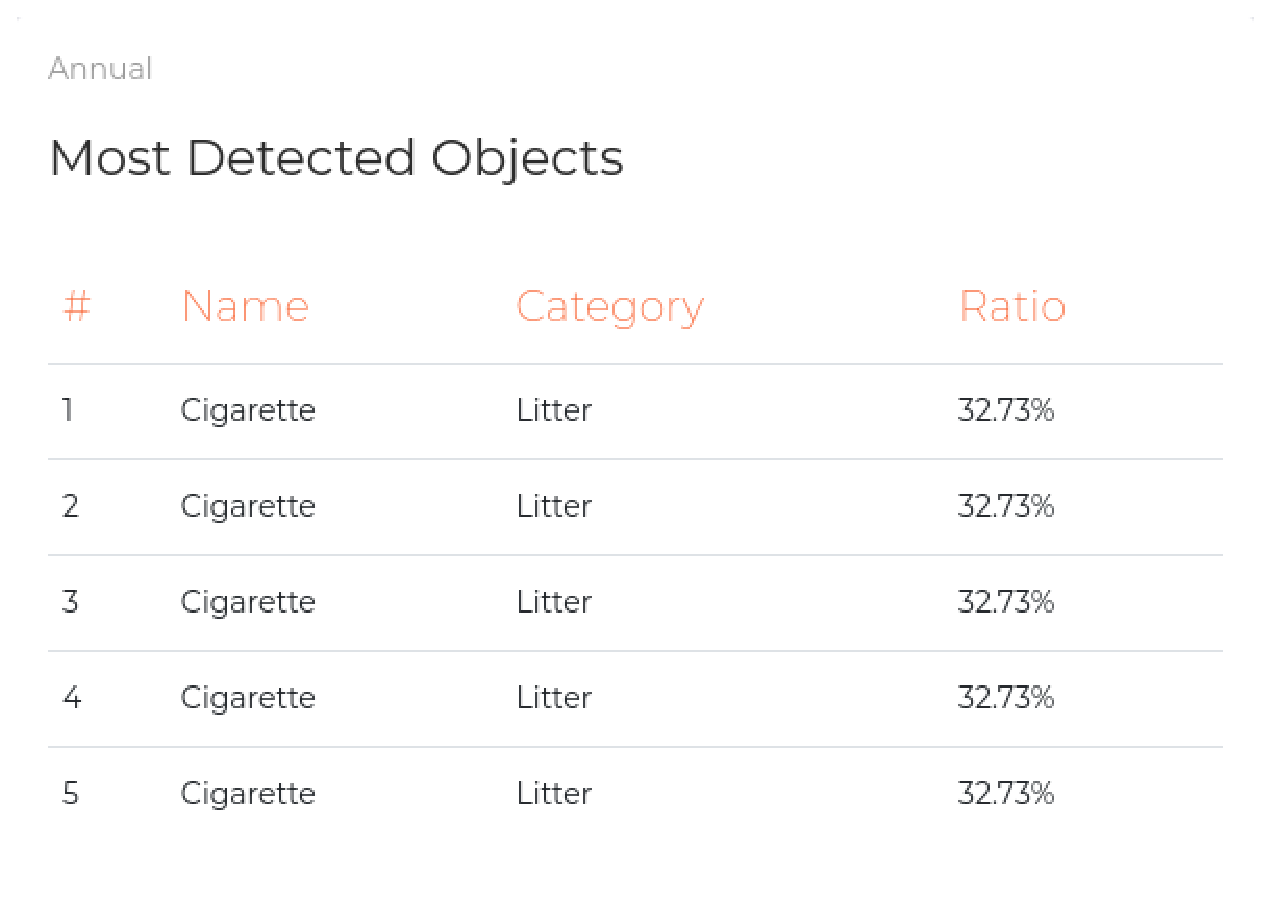
\includegraphics[width=0.48\textwidth]{images/chart_most_detected.eps}
    \caption{Most Detected Objects Table}
\end{figure}~\\

\newpage
\section{Architecture & Implementation}
\subsection{Overall Architecture & Design}
Our overall architecture consists of several major modules. At the base of our architecture lies the trained TACO model, frozen for usage in a .pb and .pbtxt format to be fed into OpenCV's DNN Module. This is linked accordingly with our C++ back-end, which is in turn, linked to our C++ Qt front-end.\\

Upon application startup, two JSON files will be read from - the config file, and the classifications file. While the config file is required to store/load user settings, the classifications file is used to store data on the various categories of objects, and respective classifications and tips. As such, on startup, the config file is read, and the settings loaded into an struct, to be referred to internally. In addition, if the database is enabled in the settings, database related information is loaded as well - the classifications are loaded into an internal map to be referred to post-inference. In addition, on database connection initiation (based on the db\_enabled setting), the existing database supercategory table is overwritten, and is loaded with the supercategory data from the classifications file.\\

In our back-end, the core centerpiece is the frozen model that is used for detections. Once a detection is triggered, an insertion transaction is conducted through a SQL wrapper class. However, as it is a real-time stream, some distinction has to be made between frames to make sure that an insertion does not occur on every single frame. As such, a rudimentary algorithm prevents this from occurring - with a frame-based cooldown being required between new detections for these detection insertion events\\

A frozen Tensorflow model is used in order to optimize inference time, with the underlying machine learning model being in the SSD MobileNet v2 architecture. The network returns several values, including the coordinates for the bounding box, the index for the detected object, and the confidence score. The main back-end handles the OpenCV instance, drawing bounding boxes around the detected object, and returning information such as what object was detected per the DNN. This information is also inserted into the database.\\

The application only does INSERT queries into the SQL, for which PostgreSQL was used. This is because the actual full statistics side (aside from the basic session statistics), is handled by the dashboard.\\

The front-end, is where the final frame - post-inference, with the object marked, is displayed. This is heavily intertwined with the front-end's Qt instance, as Qt's UI Labels are used in order to display the result of the inference (object name, class type, confidence, etc). In addition, as Qt is the main UI framework, it is used to handle the majority of user interaction, application side, such as the handling of settings, or showing session scan stats.\\

Dashboard service consists of intermediate server and front-end application. The intermediate server basically monitors the connectivity of PostgreSQL and manages connection pools. After confirming the connection is valid, it receives the  requests according to the prescribed form and executes query with the corresponding conditions. It fetches the result set and parses into JSON format.\\

The dashboard's front-end has a role to obtain the request of statistics inquiry from the user and provide the analysis information for the responses. The formats of visualization include line chart, bar chart, table and numerical figures.\\

The following diagram shows our overall architecture and application ecosystem for this project.\\

\begin{figure}[h]
    \centering
    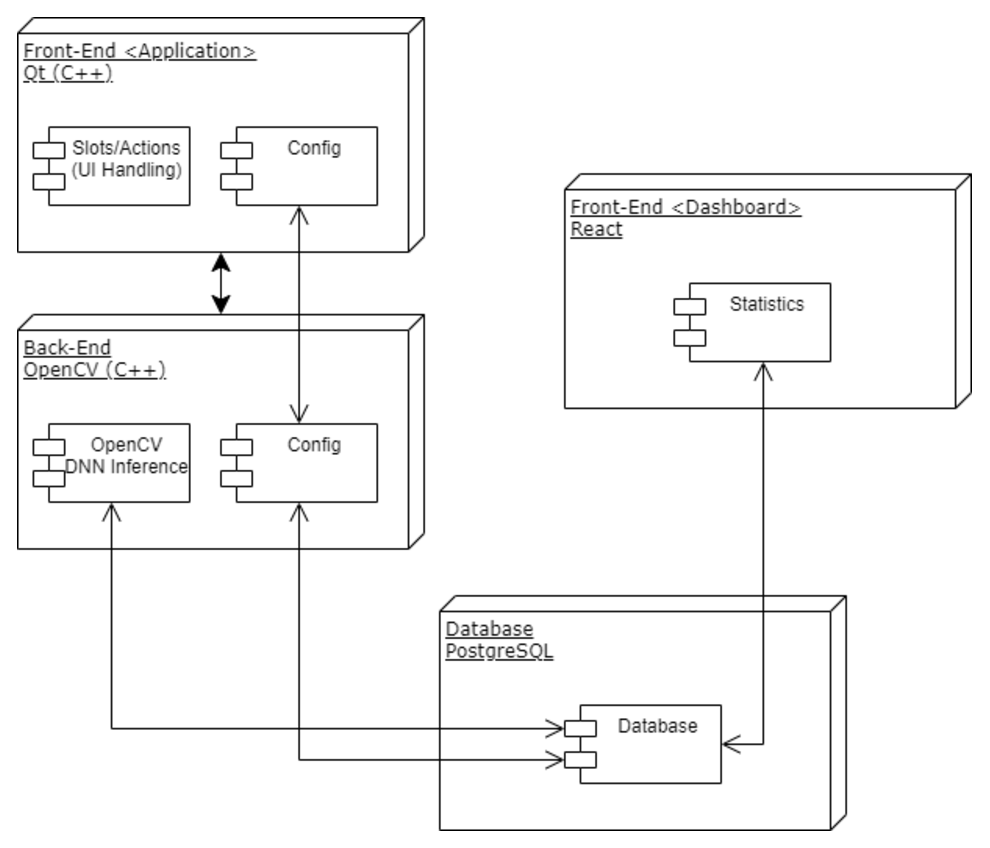
\includegraphics[width=0.48\textwidth]{images/app_diagram.eps}
    \caption{Overall System Diagram}
\end{figure}~\\

\newpage
\subsection{Database Architecture}
The following diagram shows our architecture for the database, and the source of the database data (insertion sources). Note that the dashboard is not showcased here, as the dashboard mainly only does selections from the database, and is not a source of data.

\begin{figure}[h]
    \centering
    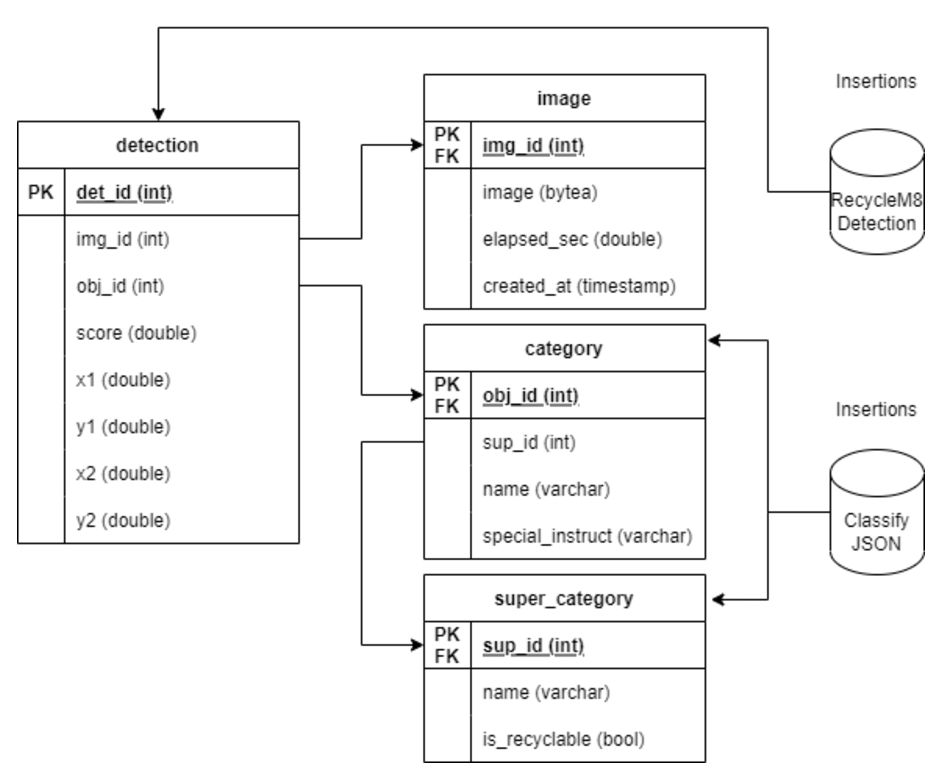
\includegraphics[width=0.48\textwidth]{images/db_diagram.eps}
    \caption{Database Diagram}
\end{figure}

\subsection{Directory Structure}
The following diagram shows our file directory structure for the application.

\begin{table}[htbp!]\normalsize
\begin{center}
\begin{tabular}{|p{1.5cm}|p{2.2cm}|p{3.9cm}|}
\hline
\textbf{Class} & \textbf{\textit{Directory}}& \textbf{\textit{Filename}}\\
\hline
Classifier & recycleAssistant & classifier.h
\newline
classifier.cpp
\\ \hline
Config Handler & recycleAssistant & confighandler.h
\newline
confighandler.cpp
\newline
\\ \hline
Database Handler & recycleAssistant & databasehandler.h
\newline
databasehandler.cpp
\newline
\\ \hline
Main & recycleAssistant & main.cpp
\newline
\\ \hline
OpenCV Handler & recycleAssistant & opencv\_handler.h
\newline
opencv\_handler.cpp
\newline
\\ \hline
RecyleM8 & recycleAssistant & recyclem8.h
\newline
recyclem8.cpp
\newline
recyclem8.ui
\newline
\\ \hline
Settings Menu & recycleAssistant & settingsmenu.h
\newline
settingsmenu.cpp
\newline
settingsmenu.ui
\newline
\\ \hline
\end{tabular}
\label{tab1}
\end{center}
\end{table}


\newpage
\begin{table}[htbp!]\normalsize
\begin{center}
\begin{tabular}{|p{1.5cm}|p{2.2cm}|p{3.9cm}|}
\hline
\textbf{Class} & \textbf{\textit{Directory}}& \textbf{\textit{Filename}}\\
\hline
Statistics Menu & recycleAssistant & statisticsmenu.h
\newline
\newline
statisticsmenu.cpp
\newline
\newline
statisticsmenu.ui
\newline
\\ \hline
Config Files & build &
classifications.json
\newline
\newline
config.json
\newline
config.json\_backup
\newline
\\ \hline
CMake & recycleAssistant, cmake & CMakeLists.txt
\newline
\newline
Findrapidjson (CMake)
\newline
\\ \hline
Libraries & dependencies & rapidjson (module)
\newline
\newline
spdlog (module)
\newline
\\ \hline
Model & build &
frozen\_taco.pb
\newline
frozen\_taco.pbtxt
\newline
\\ \hline
\end{tabular}
\label{tab1}
\end{center}
\end{table}

The components related to dashboard are described in the following diagram.

\begin{table}[htbp!]\normalsize
\begin{center}
\begin{tabular}{|p{1.8cm}|p{2.2cm}|p{3.6cm}|}
\hline
\textbf{Class} & \textbf{\textit{Directory}}& \textbf{\textit{Filename}}\\
\hline
Intermediate Server & dashboard & entrypoint.py
\newline
server.py
\newline
\\ \hline
Inquiry & dashboard & db.py
\newline
stats.py
\newline
stats\_sql.py
\newline
\\ \hline
Layout & front/dashboard & Admin.js
\newline
Dashboard.js
\newline
\\ \hline
Stats & front/dashboard & DayCntChart.js
\newline
DayRecChart.js
\newline
DayTimeChart.js
\newline
WeekUsageChart.js
\newline
\\ \hline
\end{tabular}
\label{tab1}
\end{center}
\end{table}

\newpage
\subsection{Classifier}

\begin{figure}[h]
    \centering
    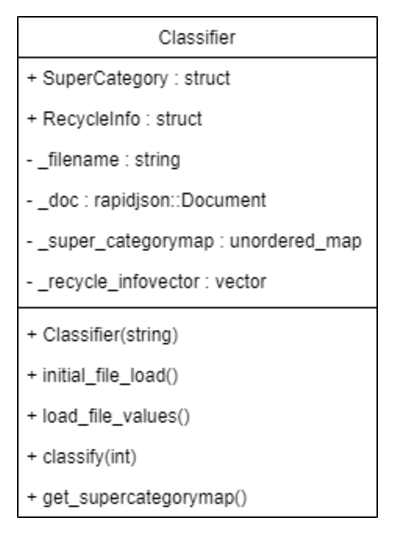
\includegraphics[width=0.35\textwidth]{images/code_diagrams/classifier_uml.eps}
    \caption{Classifier Class Diagram}
\end{figure}~\\

The Classifier Class mainly handles the classification mapping of objects. It loads data from the classifications.json file, and loads the data into a map and a vector, both of which will be referred to post-inference.\\


\textbf{classifications.json format example}~\\

The classifications.json file is the file in which the Classifier pulls all of its information from. The structure is as the following:

\begin{figure}[h]
    \centering
    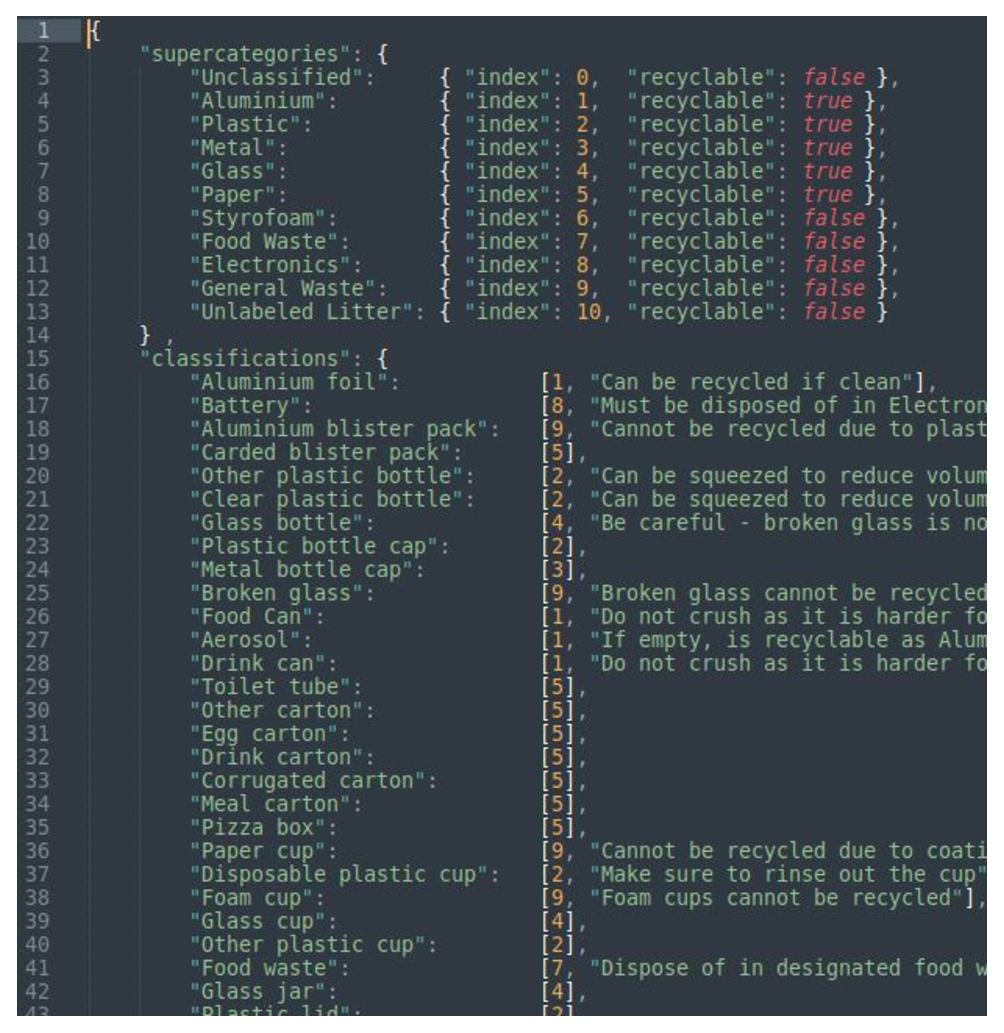
\includegraphics[width=0.48\textwidth]{images/sourcecode/classifications_json.eps}
    \caption{classifications.json sample}
\end{figure}

As noted previously, the structure follows the following format:

\begin{itemize}
\item super\_categories: object (structure below)
\begin{itemize}
\item index: int
\item recyclable: bool
\end{itemize}
\item classifications: array (structure below)
\begin{itemize}
\item int (recycling category)
\item string (recycling tip)
\end{itemize}
\end{itemize}~\\

This is the format that the Classifier expects, and will throw an error per the JSON reading/parsing code, if the format is not followed.~\\~\\


\textbf{classifier.h}~\\

The Classifier Header defines the structure of the Classifier class. It receives a filename in the constructor, but defaults to "classifications.json".

It then declares two structs, one of which is SuperCategory. This declares the ultimate recycling class, such as "Plastic", and a bool that flags if it is recyclable or not. The other struct, RecycleInfo, is per object, and declares which superclass, or supercategory it belongs to, alongside any special\_instructions that was defined in the classifications.json file. 

It defines the functions in the class, namely, initial\_file\_load(), load\_file\_values(), classify(int index), and get\_supercategorymap(), which are all public, and accessible externally.

The private variables are the data map and vectors, as they should not be modified outside of the class.~\\~\\


\textbf{classifier.cpp}~\\

In the constructor, an initialization list moves the copied argument filename into the private member \_filename. 

Then, the initial\_file\_load() function is defined, returning a bool on whether the file is valid. It returns a false if the file does not exist, and also returns a false when rapidjson encounters a parse error.

It "pre-loads" the value into a private rapidjson::Document object, so that it does not need to be loaded, or read/parsed twice later.

In the load\_file\_values() function, the values are read from the private document object. It gets the objects for both the supercategories object, and the classifications object, and parses through both of them, while packaging the data into a struct, and emplacing that into the private map or vector.

The classify function and the get\_supercategorymap exist as functions to keep the actual vector and the map private. They return the object at provided index in the vector, and a copy of the map, respectively.~\\~\\


\subsection{ConfigHandler}

\begin{figure}[h]
    \centering
    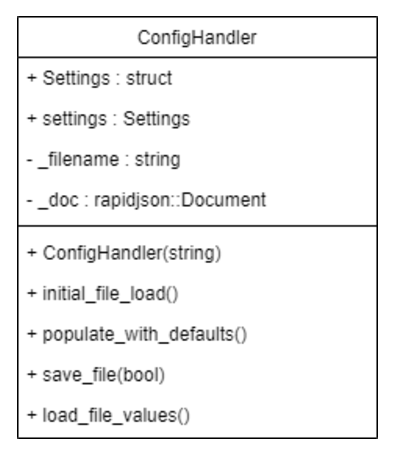
\includegraphics[width=0.35\textwidth]{images/code_diagrams/confighandler_uml.eps}
    \caption{ConfigHandler Class Diagram}
\end{figure}~\\

The ConfigHandler Class mainly handles the Configuration File - both the reading/parsing, and writing parts. It loads data from the config.json file, and loads it into a defined Settings struct.\\


\textbf{confighandler.h}~\\

The ConfigHandler Header defines the structure of the ConfigHandler class. It receives a filename in the constructor, that is used to refer to the config file.

It then declares one struct, and an object of that struct, used for settings related variables.

Several functions are also declared, initial\_file\_load(), populate\_with\_defaults(), save\_file(bool create\_new), and load\_file\_values().

Two private variables are declared - a \_filename string, and a \_doc rapidjson::Document object.~\\~\\


\textbf{confighandler.cpp}~\\

In initial\_file\_load(), a boolean is returned based on the validity of the config JSON file. If the file doesn't exist, or there is a parse error, a false is returned. In the last portion of the function, it checks to make sure the typing is correct, returning a false if the value types are parsed to be incorrect.

In load\_file\_values(), the \_settings object is loaded with the data - the data is read from the private \_doc object.

In populate\_with\_defaults(), the \_settings object is loaded with default set values.

In save\_file(bool create\_new), the private \_settings file is written to a file in a JSON format, overwriting the current config JSON file. The create\_new bool is used to flag whether it is the first save (the first creation/new creation). By default, this is flagged as false - when it is flagged false, this function will create a copy of the previous config and save it as a backup (json\_backup extension).~\\~\\


\subsection{DatabaseHandler}

\begin{figure}[h]
    \centering
    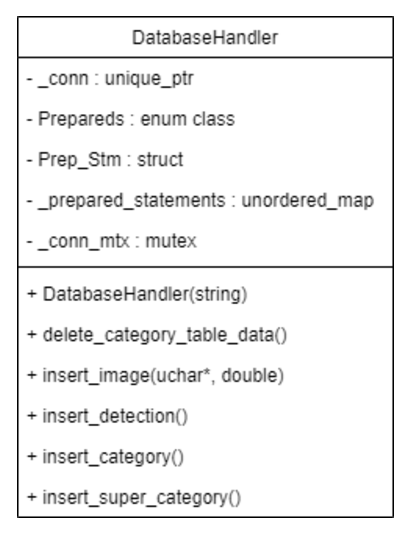
\includegraphics[width=0.35\textwidth]{images/code_diagrams/databasehandler_uml.eps}
    \caption{DatabaseHandler Class Diagram}
\end{figure}~\\

The Database Class mainly handles the Database Operations side of things for the application.\\


\textbf{databasehandler.h}~\\

The DatabaseHandler constructor is declared as accepting a connection string. Several database-related operations are declared, alongside a unique\_ptr for the connection to the database, alongside a declared enum, object and matching map, and finally, a mutex to make sure database operations are handled synchronously.~\\~\\


\textbf{databasehandler.cpp}~\\

The DatabaseHandler constructor is defined as accepting a connection string. This is used to create a unique\_ptr for the pqxx connection. Then, a nontransaction operation is declared, which is used to push the defined, prepared statements into the database connection. 

The rest of the functions in the class are C++ wrapper functions for pqxx (PostgreSQL C++ Wrapper Library) database operations. These are for various insertion operations, with the exception being a deletion operation, being used to clear the table and load in the categories into the database.~\\~\\

\subsection{Main}

\textbf{main.cpp}~\\

The main.cpp is the main function, or point of execution. Before the application is fully executed, a perform\_additional\_prestart\_actions() function is called, which is defined (and will be explained) in the RecycleM8 class.

\begin{figure}[h]
    \centering
    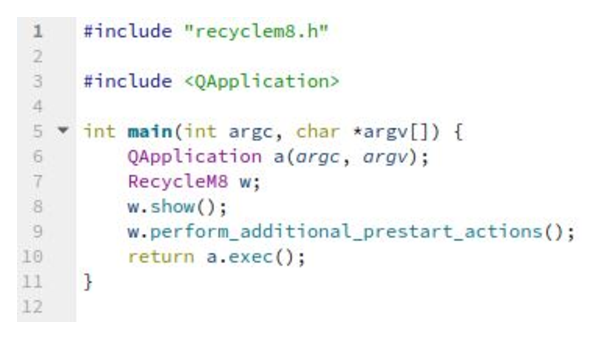
\includegraphics[width=0.48\textwidth]{images/sourcecode/main_cpp.eps}
    \caption{main.cpp}
\end{figure}~\\

The main function is kept simple, and everything happens within the called classes - in this case, the RecycleM8 class.~\\~\\

\subsection{OpenCVHandler}

\begin{figure}[h]
    \centering
    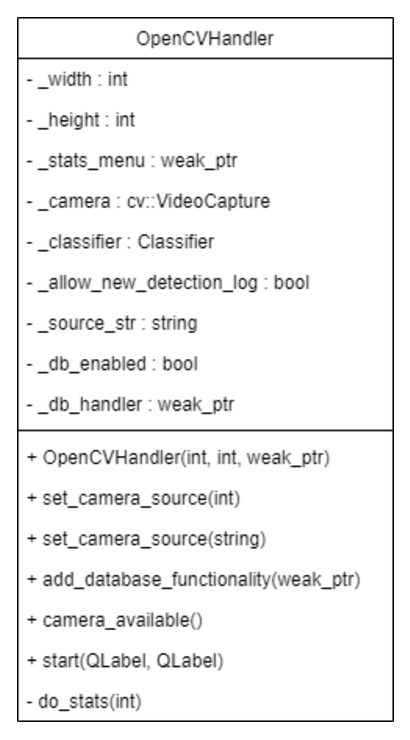
\includegraphics[width=0.35\textwidth]{images/code_diagrams/opencvhandler_uml.eps}
    \caption{OpenCVHandler Class Diagram}
\end{figure}~\\

The OpenCVHandler Class mainly handles the OpenCV and Inference side of things for the application. As the application's central focus is on this class/module, it calls a lot of references to other classes.\\


\textbf{opencv\_handler.h}~\\

The OpenCVHandler class' constructor is declared as accepting an int, and a weak\_ptr. The weak\_ptr is a weak pointer to the StatisticsMenu, as it needs to adjust values within the stats menu during scanning/detection.

Then, several functions are declared, a pair of set\_camera\_source functions, an add database\_functionality function that takes a weak pointer, and a camera\_available function, and finally, a start function.~\\~\\


\textbf{opencv\_handler.cpp}~\\

The weak\_ptr parameter in the Constructor is of the StatisticsMenu class. This is because it needs to be able to adjust the values within the stats menu (progress bars, counter, etc).

In the constructor, it also loads up the Classifier data into the private variable \_classifier. The set\_camera\_source functions create a cv::VideoCapture object, placing it in the \_camera variable. This will allow the switching of camera sources.

The add\_database\_functionality function accepts a weak\_ptr of the DatabaseHandler class. This is in order to call database related functions, mainly, insert queries when inserting data from the inference. This function is also responsible for loading up the classification data into the database (category/supercategory), deleting the pre-existing data, and replacing it with the new data.

The do\_stats function accepts an integer - referring to the index of the recycling category (ie. 1 for aluminium, 2 for plastic, etc). This will be used in a switch case statement to increment the statistics/progress bars.\\

Finally, the start function is defined, accepting two QLabels as parameters. QLabels refer to the Qt UI Labels - one of them for the actual video feed, and one of them for the classification text. For the video feed, the OpenCV frame is resized and converted into a blob, which is then forwarded into the DNN for object recognition. Based on the classification, the text (second label) displays the text accordingly, as well as inserting into the database if the database feature is enabled.

In order to prevent insertions upon every frame, a rudimentary algorithm is implemented to enforce a "cooldown" period for when new items can be inserted into the database, based on a frame-based timeout. Then, the bounding boxes are drawn on the original frame, which is then converted from a BGRA format, to a RGBA format, and a QImage is created from that color converted frame. Finally, a QPixmap is drawn from that, and the frame label is set to display that QPixmap.~\\~\\

\subsection{RecycleM8}

\begin{figure}[h]
    \centering
    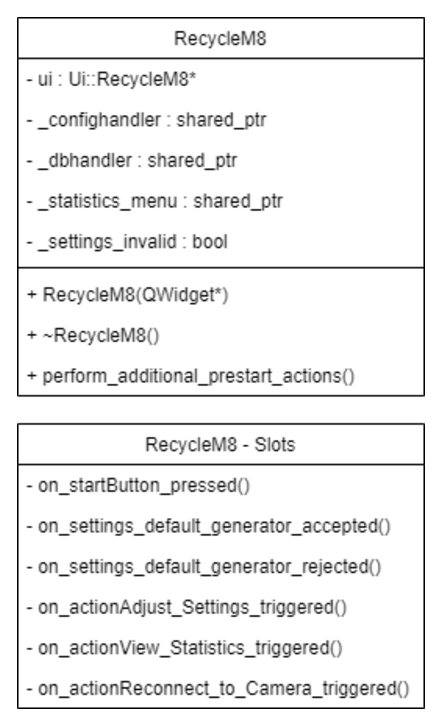
\includegraphics[width=0.35\textwidth]{images/code_diagrams/recyclem8.eps}
    \caption{RecycleM8 Class Diagram}
\end{figure}~\\

The RecycleM8 is the main entry class for the Recycling Assistant application. It mainly handles the UI flow, and ties UI elements to back-end functions.\\


\textbf{recyclem8.h}~\\

The RecycleM8 class handles mainly the UI elements, and the general flow. As such, the only other functions it calls aside from the constructor are the perform\_additional\_prestart\_actions() function, and the start\_scanner() function. In terms of variables, it holds a lot of shared pointers to other classes, such as to the Config Handling class, the Database Handling class, and the Statistic Menu class.\\

There also exist a fair amount of private \textit{slot} functions. These are linked to Qt UI elements, triggering the code inside when the action is performed. ~\\~\\


\textbf{recyclem8.cpp}~\\

In the constructor of the RecycleM8 class, the UI is setup, and the widget index is set to the start\_menu. In addition, the shared pointers for the other classes (the Config Handling class, and the Statistic Menu class) are assigned. A settings validity check is also performed, changing the value of a private boolean variable based on its result.\\


In the perform\_additional\_prestart\_actions() function, if the settings was invalid, simply returns and does not execute the rest of the function. However, if it was valid, it loads the file values, and performs further actions based on the value of some of the config flags. If the database flag was enabled, the database handler shared pointer is created, and the dashboard link is assigned. If the skip start settings flag was enabled, it sets the current widget index to the scanner and starts the scanner, thus skipping straight to the scanner/detection screen.~\\~\\

\subsection{SettingsMenu}

\begin{figure}[h]
    \centering
    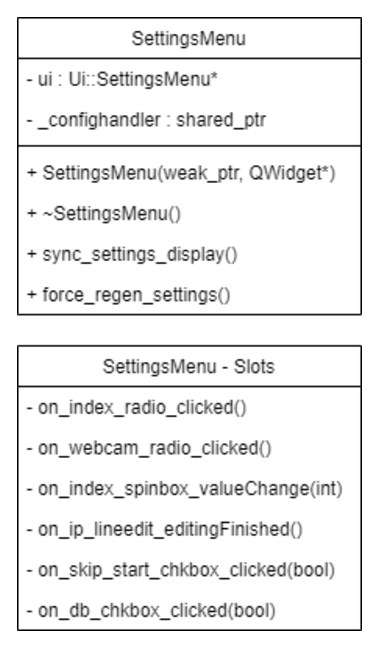
\includegraphics[width=0.35\textwidth]{images/code_diagrams/settingsmenu.eps}
    \caption{SettingsMenu Class Diagram}
\end{figure}~\\

The SettingsMenu handles the Settings/Config UI end of the application, saving new values to the config file and syncing changes made on the UI, to the config file.\\


\textbf{settingsmenu.h}~\\

The SettingsMenu header declares the constructor, a custom destructor, two public functions, and a weak pointer in addition to the default Ui pointer. The constructor accepts a weak pointer of the ConfigHandler class as a parameter, and a QWidget parent pointer. ~\\~\\


\textbf{settingsmenu.cpp}~\\

The SettingsMenu code mainly focuses around handling UI elements, and linking them into actions. A general sync settings display function is used in order to "sync" UI elements to the values that are currently loaded into the settings. This means that the settings menu will not be a fresh state, but will reflect the currently applied settings.\\

In addition, the other settings modify the values in settings, which will be reflected across the application due to the weak pointer link to the ConfigHandler, that other parts of the application also utilize. Every action also calls a save file function, thus writing the new settings state to the config file.~\\~\\

\subsection{StatisticsMenu}

\begin{figure}[h]
    \centering
    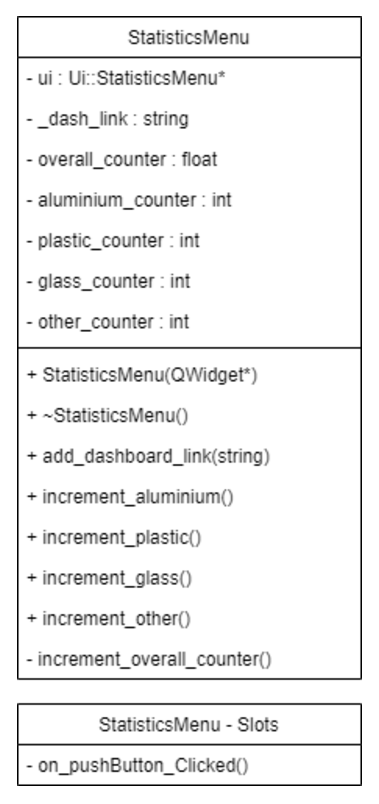
\includegraphics[width=0.35\textwidth]{images/code_diagrams/statisticsmenu.eps}
    \caption{StatisticsMenu Class Diagram}
\end{figure}~\\

The StatisticsMenu handles the Statistics UI end of the application, displaying progress bars and a counter designed to represent the type of objects detected. In addition, an extra tab exists to link to the dashboard.\\


\textbf{statisticsmenu.h}~\\

The StatisticsMenu header declares the constructor, a custom destructor, two public functions, and a weak pointer in addition to the default Ui pointer. The constructor accepts a weak pointer of the ConfigHandler class as a parameter, and a QWidget parent pointer. There are several incrementing functions declared, with matching variables, a private void function that increases the overall counter. There is a single private slot, used for linking the user to the dashboard.~\\~\\


\textbf{statisticsmenu.cpp}~\\

The StatisticsMenu code mainly focuses around displaying and managing the basic statistics of the application. An increment overall counter function is made private, which increases the overall\_counter float - this is called within all the other increment functions. These other increment functions work on the basic premise that if for example, an aluminium can is detected, +1 to the aluminium counter, but +1 to the overall as well. The overall\_counter here is set to a float to prevent loss of precision (ie. 0.5 being converted to 0). The increment overall counter function also performs some basic math to convert these values into a percentage out of 100, rounding up, to be fed into the progressbar values. At the same time, it also increases the label for the overall scan count. This means that it serves a dual function of both incrementing the overall\_counter variable, but also updating the display for all progressbars.\\

The on\_pushButton\_clicked function is only available if there is a set \_dash\_link (dashboard link), set within the settings. If it is not empty, then it will open up browser window linking the user directly to the dashboard link.~\\~\\

\subsection{Dashboard}

\textbf{server.py}~\\

Dashboard's intermediate server has a responsible for interactions between Frontend and PostgreSQL. It receives the request via WSGI framework within the predefined API rules. It communicates with the PostgreSQL through psycopg2 adapter in order to make inquiry to the DBMS. It basically checks the database status and maintain the connection pools created at the launching.~\\

\textbf{stats.py}~\\

Dashboard stats code mainly focuses around interpret the request parameter and executing the query. It decides which prepared statements should be used for given requests and assign proper condition variables of period range or another specific condition of the analysis. After preparing the query statement, it obtains an available connection from the connection pool. After finishing the execution, it parses the result into dictionary and JSON format. It returns the no longer used connection to the pool.~\\

\textbf{Dashboard.js}~\\

It maintains the parameters from the user and contains the overall visualized reports and their layout. It holds the statDate variable to determine the analyzing years, months and days. When a user tries to inquiry the dashboard, it makes multiple requests to the intermediate server. Those requests are handled in asynchronously with their own callback functions for each.\\

The dashboard layout consists of multiple line graphs, bar graphs and tables. All graphs and tables are located in the sections, with a header and footer for each box areas. Chart components have their own visualization options such as background color, line style and grid style. This configuration is applied when the graph is drawn on the canvas element.~\\~\\

\section{Use Cases}

\subsection{Opening The Application}~\\
\texttt{Requirement A}~\\
\subsubsection{Expected}~\\
When the application is opened, the main start screen should appear, unless the user has specified that the application should skip straight ahead to the detection screen in the Settings Menu. If the user's config file is corrupted, or it is their first launch, it should also direct the user to the main start screen.~\\

\subsubsection{Result}~\\
The application meets the specification, and follows the UI flow according to the Expected Result.

\begin{figure}[!h]
    \centering
    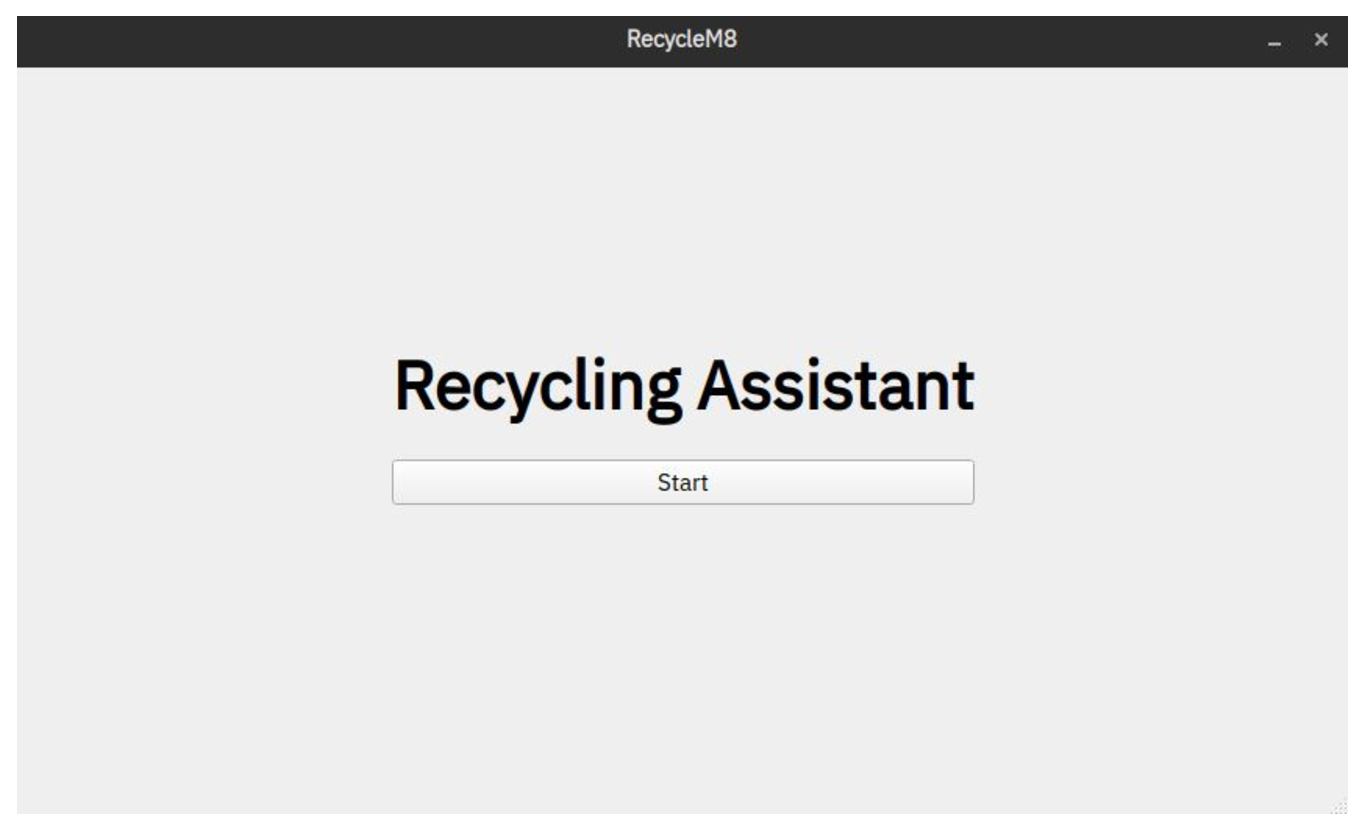
\includegraphics[width=0.35\textwidth]{images/start.eps}
    \caption{Default (no skip), or corrupted/first launch}
\end{figure}

\begin{figure}[!h]
    \centering
    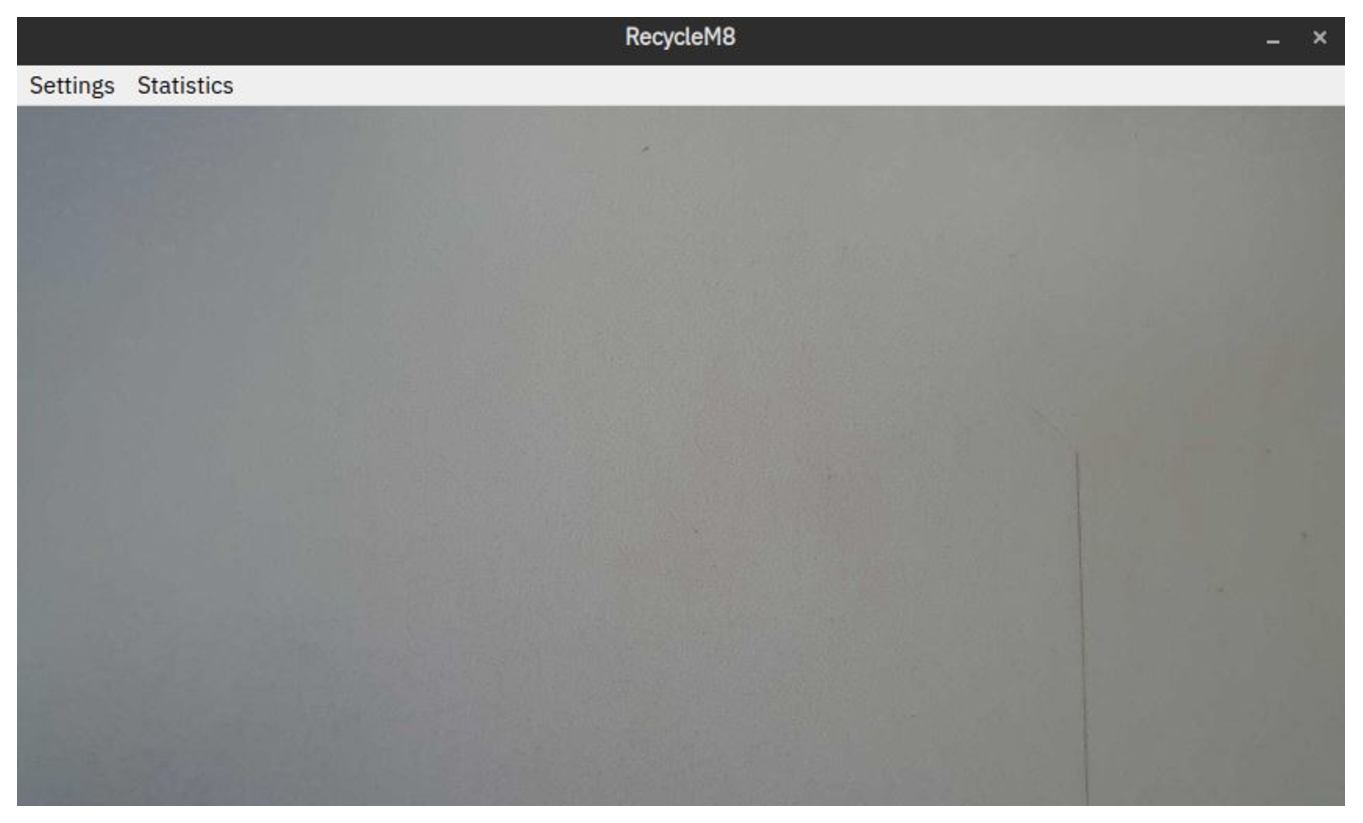
\includegraphics[width=0.35\textwidth]{images/nothing_detected.eps}
    \caption{User specified skip to detection on startup}
\end{figure}~\\

\subsubsection{Use Case}~\\
When the application is first opened, the application checks for the existence of a config file, checking the validity of the values inside of the config file if it does exist. Amongst the various config/settings flags, if the user has opted to skip the "startup" phase, they will be skipped directly to the detection screen.\\

However, if they have not, or it is their first start up, the user will be greeted with a basic screen with a "Start" button, which is centered in the middle of the screen, right below the title "Recycling Assistant". Once the user clicks it, they will be brought to one of two screens based on the config validity/existence. \\

If the config file does not exist or is not valid, the user will be brought to a screen in which they will be prompted to regenerate the config file with default parameters. If the user clicks Okay, the settings file will be populated with default parameters, and they will finally be brought to the detection screen. If the user clicks Cancel, they will be brought back to the title/previous screen. \\

If the user's config file existed and was valid, they will also be brought to the detection screen after pressing the "Start" button.~\\

\subsection{Input Support}~\\
\texttt{Requirement D}~\\
\subsubsection{Expected}~\\
The application should be able support a real-time input of a physically or local network connected camera. If the input is not detected/invalid, the user should be notified.~\\

\subsubsection{Result}~\\
The application meets the specification, and can support both a locally connected physical camera, or a network connected webcam camera. If the input is not detected or valid, the application notifies the user through an error message.

\begin{figure}[!h]
    \centering
    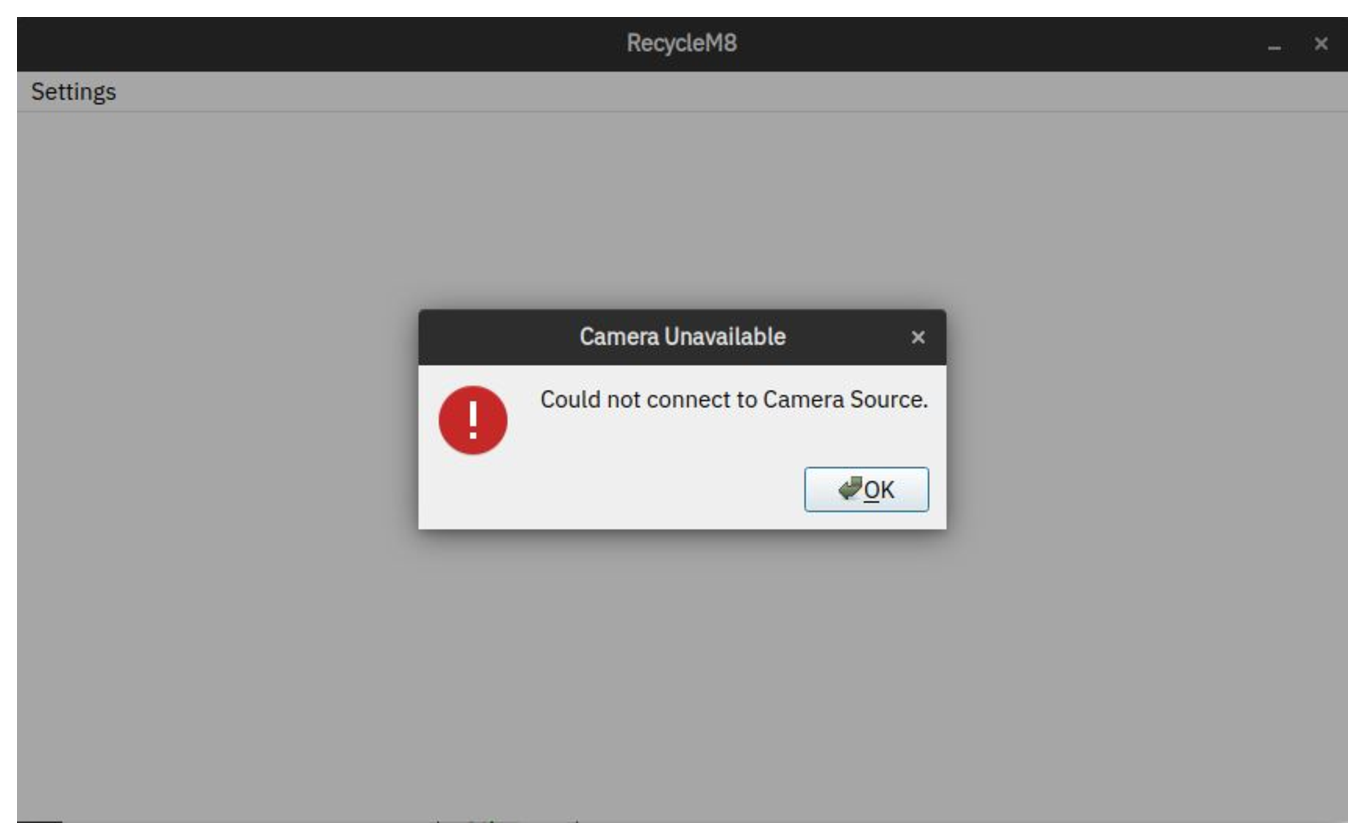
\includegraphics[width=0.35\textwidth]{images/camera_source_error.eps}
    \caption{Camera Not Detected Error Message}
\end{figure}~\\

\subsubsection{Use Case}~\\
When the user encounters the detection screen, a scanner instance will be opened based on the camera feed specified. That camera feed will be then displayed as a majority of the window, in real-time, in the correct color. However, if the user's camera source was unavailable or invalid, they will see an error message, notifying them that the application was not able to connect to their specified camera source. It is a modal window, which also greys out the background, so they cannot take any action without acknowledging the message. \\

The user is expected to check their settings in the settings menu and use the reconnect context menu action to establish a connection again. Otherwise, they will be looking at a screen that simply notifies the user that the application is not connected to anything.~\\

\subsection{Real Time Analysis}~\\
\texttt{Requirement E ~ H, L}~\\
\subsubsection{Expected}~\\
The application should be able to handle real-time detection, as well as be able to analyze and classify the object, drawing bounding boxes and text where necessary. In the text, some explanation or tip should be included regarding the detected object's recyclability candidacy. If there are multiple objects detected in the frame, they must also be drawn appropriately.

The application should also showcase additional statistics, such as the confidence level/score of the detected object/inference result, in order for insertion into database.~\\

\subsubsection{Result}~\\
The application meets the specification, using a frozen SSD MobileNet v2 inference graph in order to handle real-time detection/inference. It classifies the object based on the visual input, and draws a bounding box and uses a QLabel to write out the corresponding text based on the returned inference data - the user receives textual feedback based on the object detected. In addition, the confidence level/score is outputted.\\

Based on the detected object, a stored tip defined in the Classifications.JSON file is provided. Multiple object detection is also handled, drawing boxes around several objects where applicable. \\

\subsubsection{Use Case}~\\
In the detection screen, inference is running on every frame that is processed. When the user points the camera, or the camera is shown an object that the neural network recognizes, an output is shown. The definition "recognizes" refers to the neural network recognizing an object with a certain degree of certainty (ie. 50\% certain). \\

A bounding box is then drawn around the object, with a corresponding text box showing up in the bottom center, containing information on the detected object, the recycling class, confidence score, and stored tips in relation to the object. This textbox is hidden for when nothing is "recognized", so that there isn't an empty textbox randomly in the feed, but triggered to show upon a recognition event.~\\
 
\begin{figure}[!h]
    \centering
    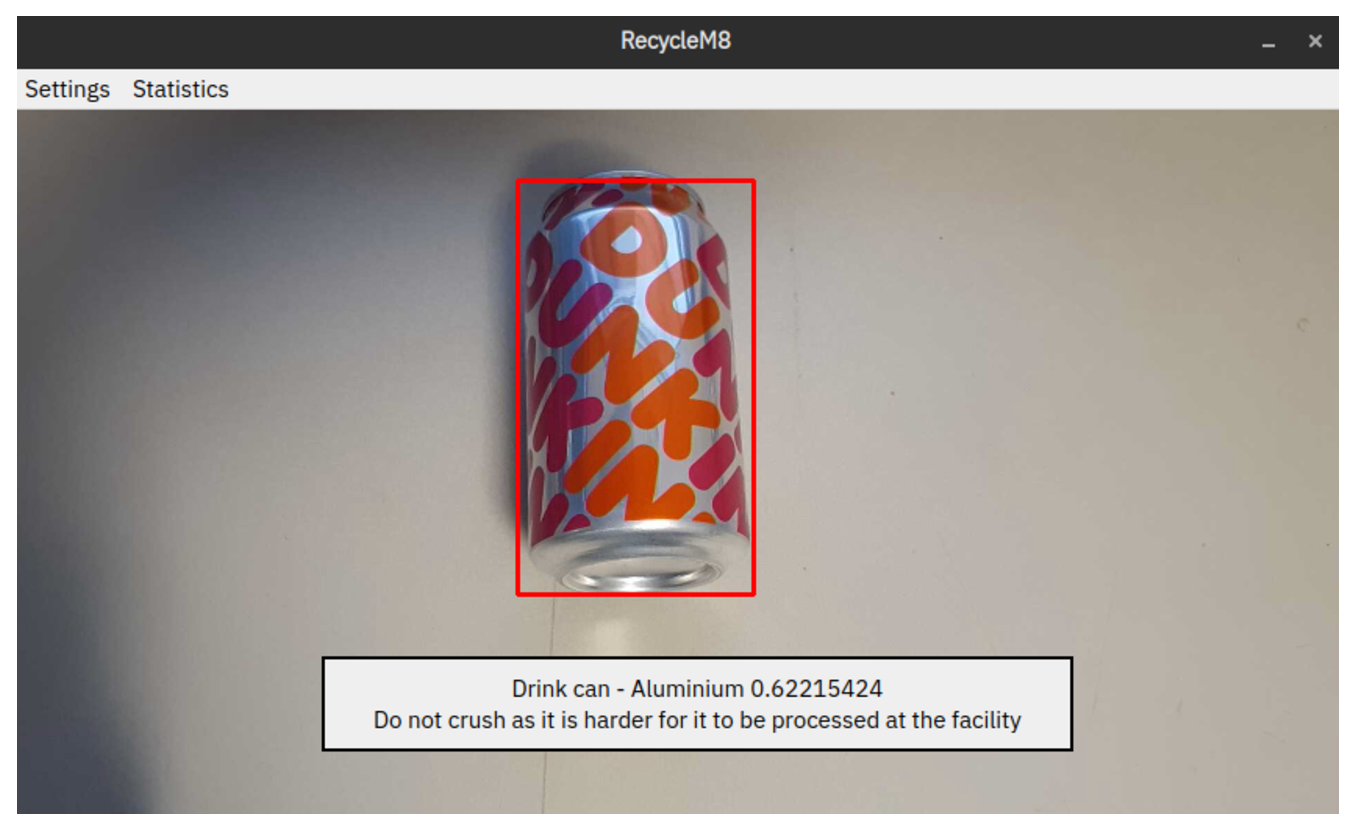
\includegraphics[width=0.35\textwidth]{images/successful_detection.eps}
    \caption{Real Time Analysis}
\end{figure}~\\

\subsection{Failure to Detect}~\\
\texttt{Requirement I}~\\
\subsubsection{Expected}~\\
If the application does not see an object, it should not trigger a detection event.~\\

\subsubsection{Result}~\\
In order to meet this specification, the baseline required confidence level in order to trigger a detection event was implemented. As a result, if the confidence level is below a specified level, it will not trigger a detection event.

\begin{figure}[!h]
    \centering
    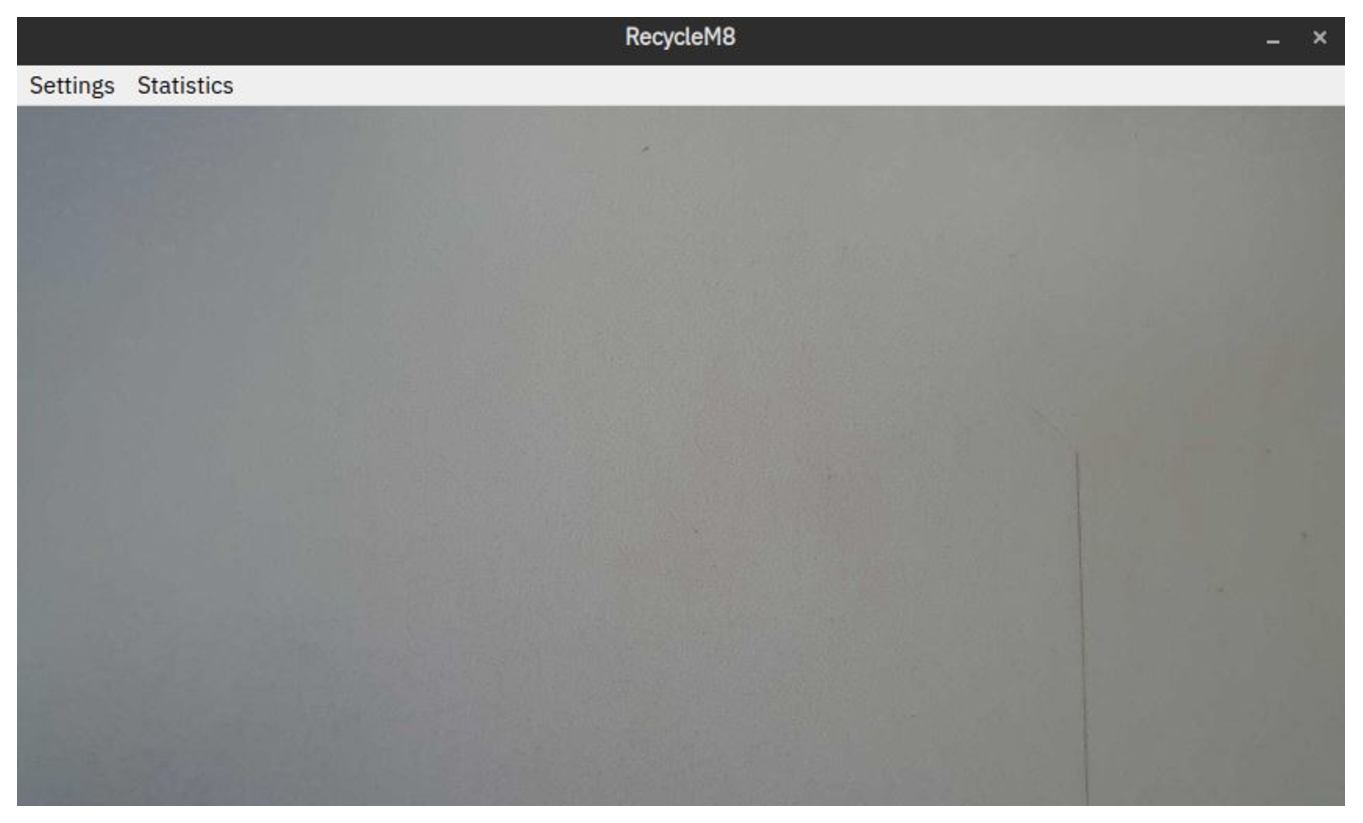
\includegraphics[width=0.35\textwidth]{images/nothing_detected.eps}
    \caption{No Detection Triggered}
\end{figure}~\\

\subsubsection{Use Case}~\\
As specified previously, certain UI elements or bounding boxes are not drawn if the confidence score hits above a set threshold. When this is the case, no bounding boxes are drawn, and the textbox for where the user receives the object's name, class, score, etc, is hidden.~\\

\subsection{Database Functionality}~\\
\texttt{Requirement J}~\\
\subsubsection{Expected}~\\
A local database should be able to be inserted into, storing data such as the timestamp, detected object, object classification, object categorization, confidence level, picture. This database should be accessible by the user to see data such as the most frequently detected category.~\\

\subsubsection{Result}~\\
In order to meet this specification, the user has the option to link a PostgreSQL database to the application. If the database function is then enabled, when a detection is made, the data from that is inserted into the DB, with the specified data.

It is accessible normally by the user, as it is a PostgreSQL database.

\begin{figure}[!h]
    \centering
    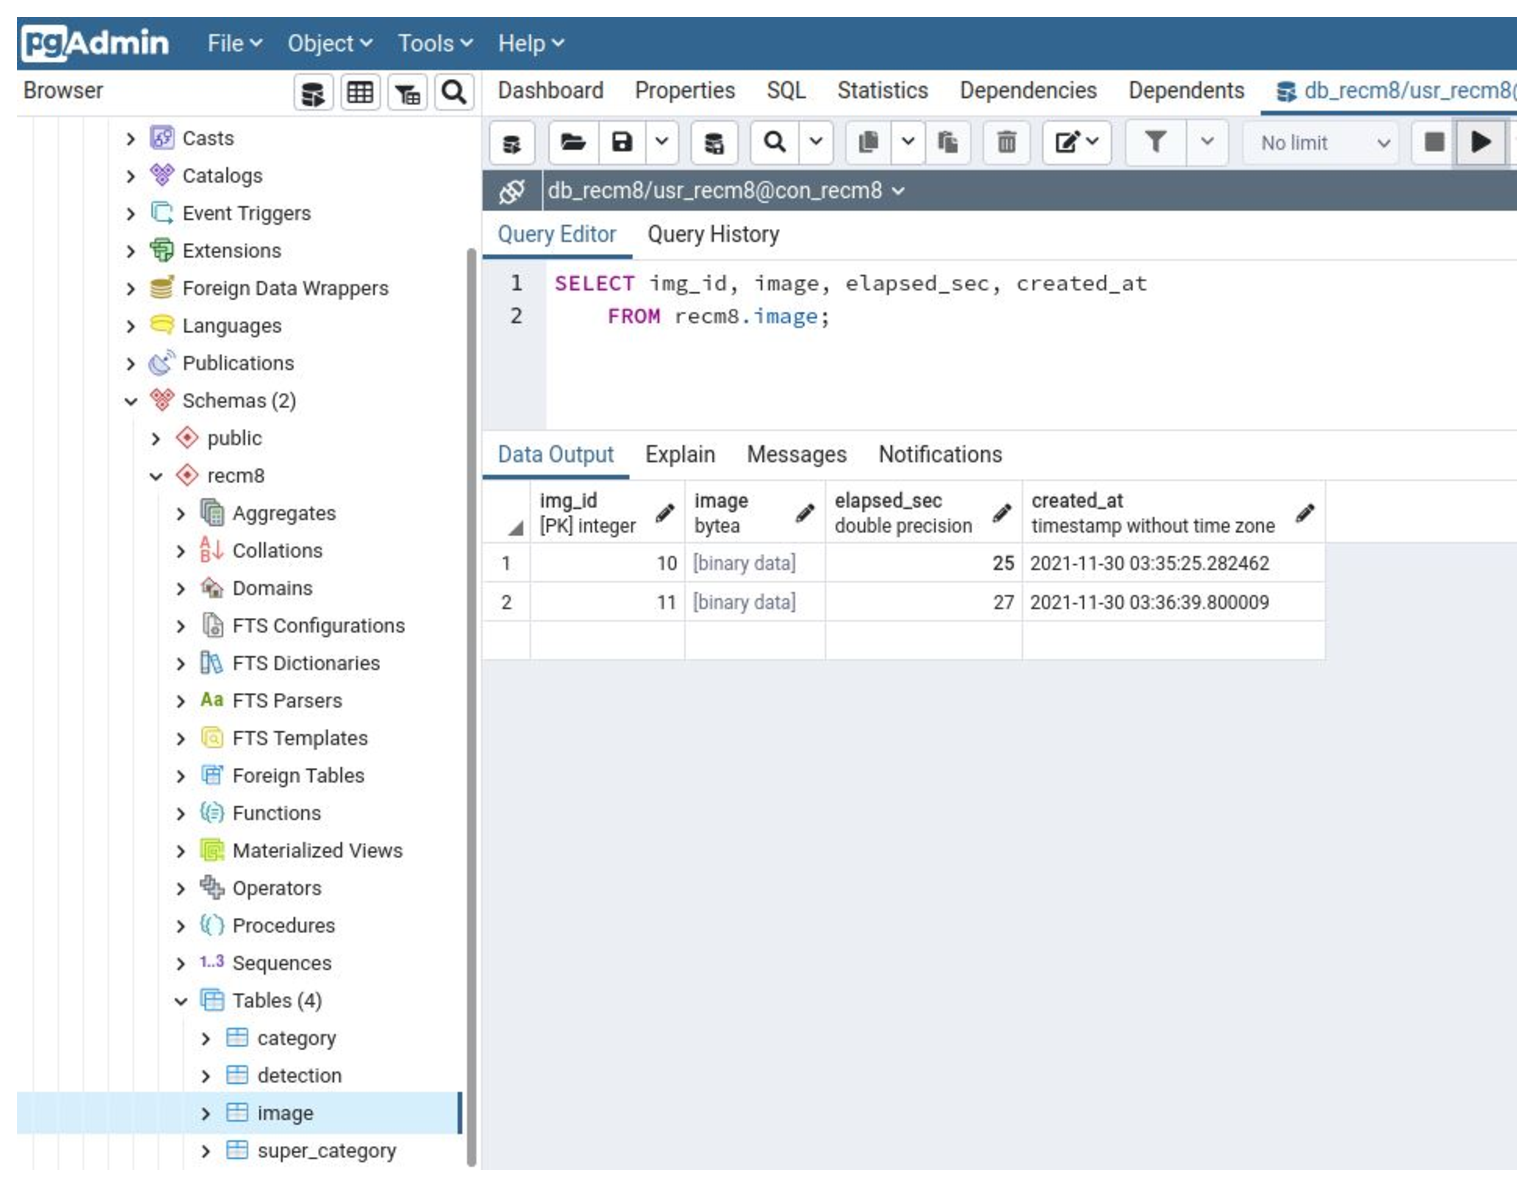
\includegraphics[width=0.35\textwidth]{images/code_diagrams/pgadmin_db.eps}
    \caption{PostgreSQL Admin}
\end{figure}~\\

\subsubsection{Use Case}~\\
When the database is enabled, the application pushes a set of base data into the database - the categories and supercategories. For images and detections, this data is pushed upon detections, with a timeout structure. This data can be viewed in the pgAdmin dashboard, or the application's dedicated statistics dashboard. 

\subsection{Statistics}~\\
\texttt{Requirement K}~\\
\subsubsection{Expected}~\\
Basic statistics should be available, such as overall detection count, count per category, etc. Session's detections should be a separate option from overall detections, and a statistics menu should be available via a UI element on the main screen.~\\

\subsubsection{Result}~\\
The application comes with a built-in session's statistics menu, representing the data with an overall counter and various progressbars. This menu is accessible via a UI context menu element. In the same window, a tab can be utilized to lead the user to the dashboard, where the overall data is shown - which requires the database functionality to be enabled.~\\

\subsubsection{Use Case}~\\
When the database is enabled, the application pushes a set of base data into the database - the categories and supercategories. For images and detections, this data is pushed upon detections, with a timeout structure. This data can be viewed in the pgAdmin dashboard, or the application's dedicated statistics dashboard. \\

In the application's statistics window, which is accessible through the Statistics Context Menu, the user can open a Statistics window that is non-modal. This means that the user can still see and interact with the main window with the statistics window open. \\

In the Session Stats, there is a "Session Scan Count" label, and four progress bars with percentage labels below that, titled "Categorical Scan Count". For example, if a Plastic Bottle is scanned, the Session Scan Count will be incremented, and the Plastic progress bar will be incremented in accordance to how many items scanned so far, were plastic.\\

In the Overall Stats tab, the user will see text notifying the user that the database function needs to be enabled, and a button below the text. The button will lead the user to the dashboard - opening the browser, and linking directly to the dashboard link set in the config.\\

\begin{figure}[!h]
    \centering
    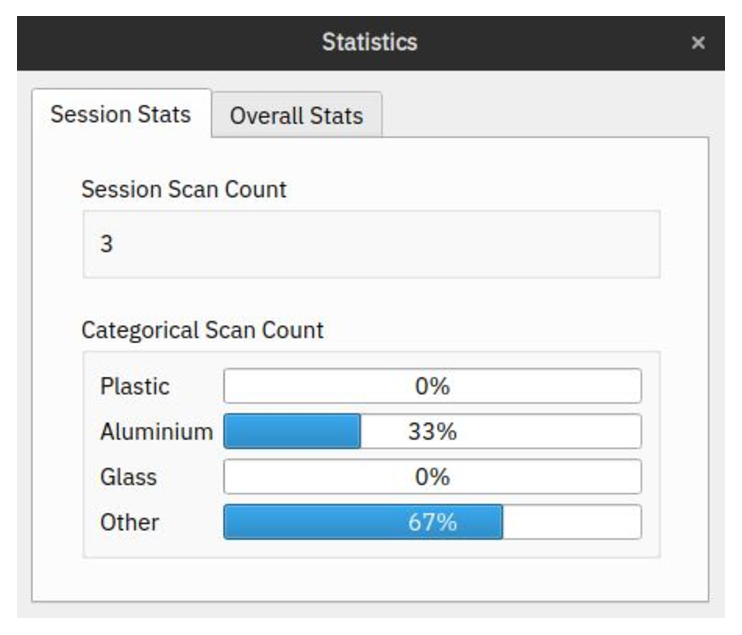
\includegraphics[width=0.35\textwidth]{images/filled_session_stats.eps}
    \caption{Basic In-App Statistics}
\end{figure}~\\

\newpage
\subsection{Settings}~\\
\texttt{Requirement B}~\\
\subsubsection{Expected}~\\
The application should come with a set of default or baseline settings, which should be editable through a settings context menu button.~\\

\subsubsection{Result}~\\
The application meets the specification, and has an implemented a settings context menu button, and a settings window in which the user is able to change their settings.

The application does come with default settings, allowing the user on first startup to generate a config file with default parameters, or also allowing the user to revert to default settings in the event that their config file seems to be either invalid, or corrupted.

While data corruption/invalidity is dealt with with the prompt to generate new default parameters, whenever the file is written to, a backup is made of the previous settings - this fits in line with the requirements laid out in Requirement B.~\\

\subsubsection{Use Case}~\\
The settings window is accessible through the main windows' context menus. Once it is open, there are three tabs, one for Application related settings, OpenCV related settings, and finally, Database related settings. In the OpenCV tab, there is a group of two radio buttons, specifying between physical, or web connected cameras. Based on this selection, the OpenCV connection will be opened using the value specified in the below index spinner (if physical is selected), or the value specified in the below text field (if webcam is selected).\\

In the Application Settings tab, there is a single checkbox option available, related to the start sequence of this application. If this is toggled, the application will skip the start sequence - skipping directly to the detection screen upon application startup. If this is not toggled, the application will go through the normal start, going to the "title" screen, requiring the user to press the "Start" button to continue onto the detection screen.\\

In the Database Settings tab, there is a single checkbox option available, related to the database portion of the application. If this is toggled, the application will link with the database specified in the connection string parameter in the config, causing detections to trigger insert queries. This requires a database to be installed, and enabled.\\

\begin{figure}[h]
    \centering
    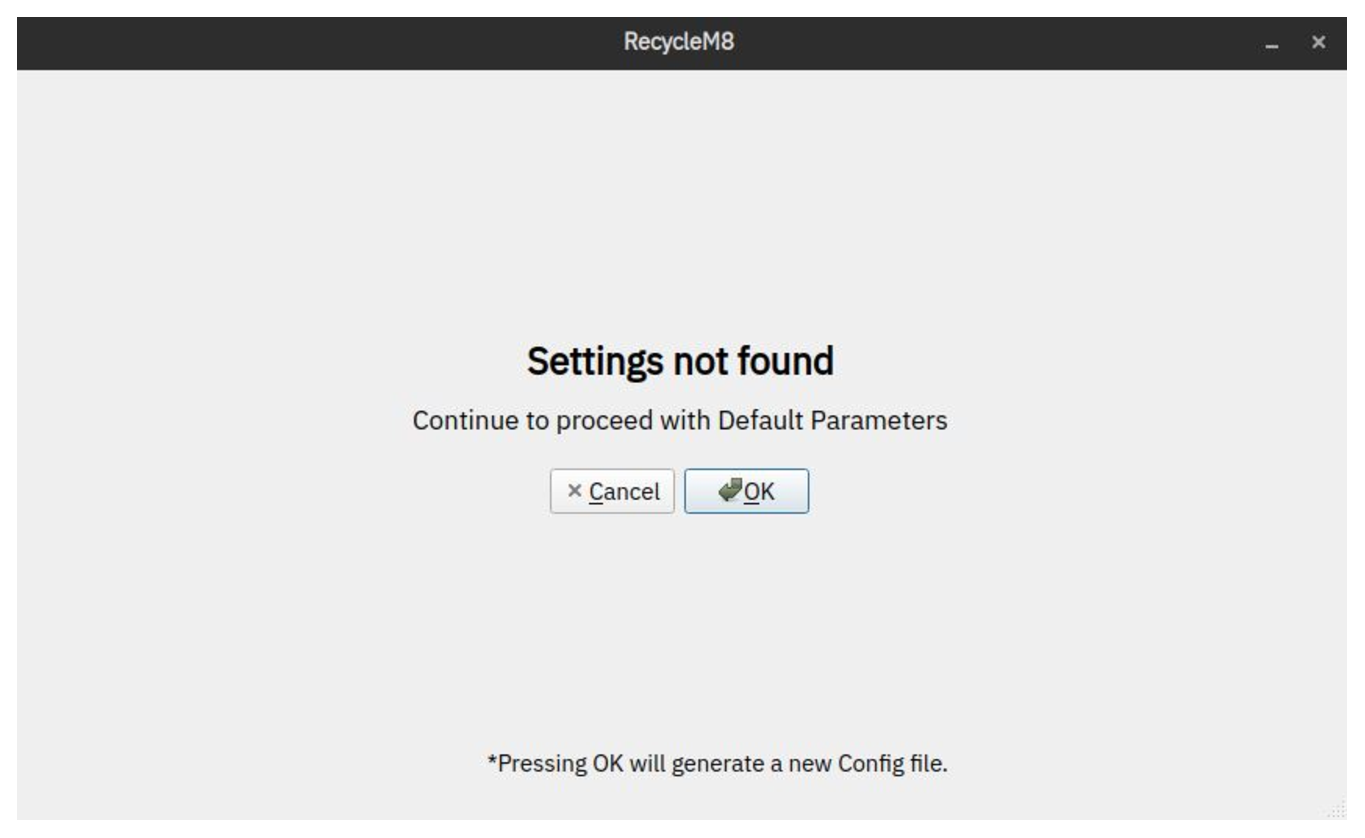
\includegraphics[width=0.35\textwidth]{images/settings_alert.eps}
    \caption{Generate Default Settings}
\end{figure}

\begin{figure}[h]
    \centering
    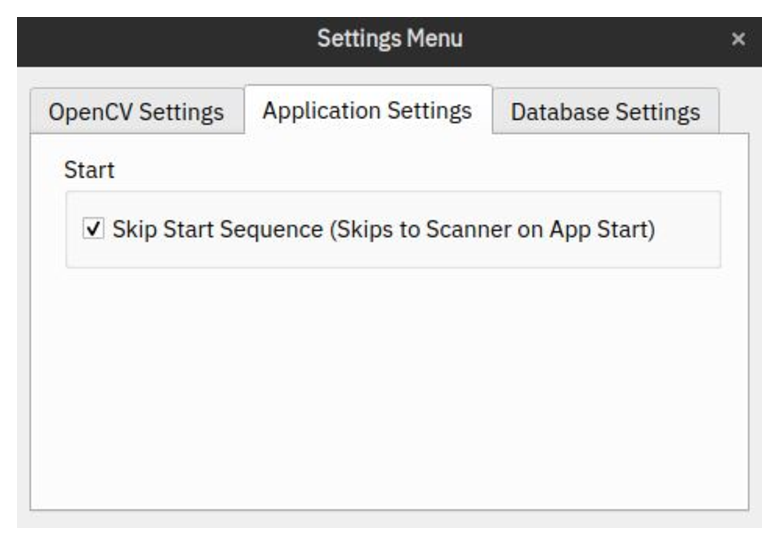
\includegraphics[width=0.35\textwidth]{images/app_settings.eps}
    \caption{Application Related Settings}
\end{figure}

\begin{figure}[h]
    \centering
    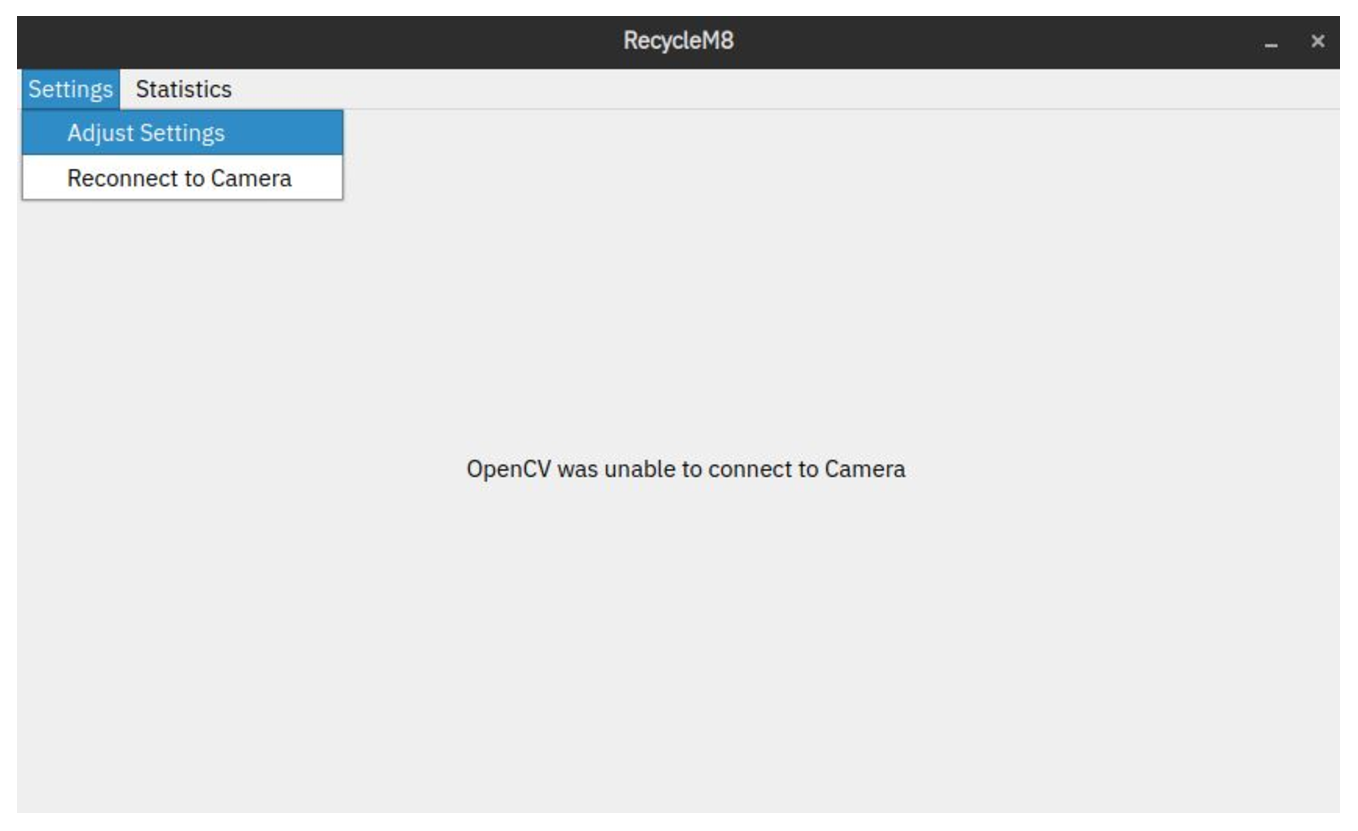
\includegraphics[width=0.35\textwidth]{images/adjust_settings.eps}
    \caption{Adjust Settings Window}
\end{figure}~\\

\newpage
\subsection{Exiting the Application}~\\
\texttt{Requirement C}~\\
\subsubsection{Expected}~\\
The user should be able to exit the application normally, and smoothly, with minimal chance of data corruption.~\\

\subsubsection{Result}~\\
The application meets this basic specification, allowing the user to quickly exit the application without any interruption or confirmation message required. The Settings Implementation reduces chances of data corruption, also allowing the opportunity for the user to recover their data in the event that it does get corrupted.~\\

\subsubsection{Use Case}~\\
When the user has control of the main application, the user may click the "x" at the top right corner to exit out of the application at any time. The only conditions where this is not fully applicable, is where a modal window is open (ie. Error message popup).\\

\subsection{Dashboard}~\\
\texttt{Requirement P, Q}~\\
\subsubsection{Expected}~\\
The user should be able to see the detailed statistics that analyzed data within the given conditions.~\\

\subsubsection{Result}~\\
In order to display the statistics, the intermediate server and front-end application are launched before the usage. The connections between PostgreSQL and intermediate server, and between intermediate server and front-end are linked successfully. When there is the actual request to load the dashboard, All graphs and tables should be displayed with correct precision and range.~\\

\subsubsection{Use Case}~\\
Before the user wants to look up the dashboard, an interactive server has been already running. As the main application is opened, the connections to the PostgreSQL is succeeded and the connection pool is created by the set number in the configuration file. If it is failed to connect the DBMS, it prompts the fail log on the console and waits until the new request is received.\\

While the intermediate server is launching, the front-end application is also started. It reads the predefined intermediate server's address and port and keeps them for the future operations. After the all steps of start up are proceeded, the dashboard leads the access user to the admin layout page.\\

\begin{figure}[h]
    \centering
    \includegraphics[width=0.35\textwidth]{images/dashboard_init_page.eps}
    \caption{Initial Dashboard Window}
\end{figure}

The initial dashboard page's statistical parameter is configured for the current day and hour. The current time is determined by the time of the browser which the user accesses through. It renders the analysis date in the middle of the page and its format contains year, month and day.\\

When a user try to change the analysis date, it can be done by two ways. The first method is click the box of date. The page will shows the calendar of the configured date's month. A user can change the months by clicking the arrows located in both left and right side. The year can changed by clicking the dropdown box on the top of calendar. After the user finds the day and clicks the it on the calendar, the chosen date's year, month and day are applied to the box of analysis date. Another way is clicking one of numbers in the box, then typing the year, month and day matching the date format.\\

\begin{figure}[h]
    \centering
    \includegraphics[width=0.35\textwidth]{images/dashboard_change_date.eps}
    \caption{Dashboard Change Date}
\end{figure}

When the user changes the analysis date or initially opens the dashboard, the requests for updating the graphs and tables are sent to the intermediate server. All data required to update the window is sent for each dataset in asynchronously. After the intermediate server receives the requests from the front-end application, it parses the parameters enclosed in the request path. The string format of statistics date will be parsed as yyyyMMdd format. If the type or format of parameter is not matched, it will be assigned to the default variable.\\

After the server module finishes to parse the parameter and finds the statistics functions corresponding to the requests, the methods of stats module are called. The stats function initially finds a specific prepared statement in the stats\_sql module. It obtains a connection from the pool. If the execute statement is SELECT query, it also obtains a cursor from the connection.\\

After all preparations are ready to execute a query, db module calls the execute method of the connection. If the statement is UPDATE clause, the transaction is commited if the call is successful. For the SELECT query, it fetches the result set to the cursor obtained before. All rows in the cursor are converted into the list of dict object. If there is no result, empty array is returned.\\

The dictionary type of analysis result is parsed in JSON format on the intermediate server. The front-end application receives the response in JSON. If the received data is used in the line or bar graph, it is passed to the corresponding Chart object's constructor. Then the object assigns the attributes of x, y labels and values. The chart option is also assigned inside the constructor.\\

\begin{figure}[h]
    \centering
    \includegraphics[width=0.35\textwidth]{images/dashboard_response_json.eps}
    \caption{JSON from Intermediate Server}
\end{figure}

The created chart objects are displayed for each assigned layout. If the chart has no available values, it shows empty space. Otherwise, the chart first limits the y axis range encompassing y values, and puts all lines or bars on the matching x axis for each. When a user hovers the dot or box of graph, it displays the label name, x value and y value until the mouse out event.\\

\begin{figure}[h]
    \centering
    \includegraphics[width=0.35\textwidth]{images/dashboard_hover.eps}
    \caption{Hover on the graph}
\end{figure}

The graph of daily counts per super categories is shown in the line plot. To make an analysis, it collects all images inserted during the 0 AM to 23 PM of the analysis date. For each captures, the statistics inquiries the corresponding detections that contain the detected objects' names and finds their super categories' names. After all information is found, it takes top 3 most detected super categories' names and their counts per hour. If there is no detection of the specific hour and super category, the empty rows' counts are considered as zero. Before returning the analysis result, it converts the y axis basis to the x axis format in order to fit the matching front-end's format.\\

\begin{figure}[h]
    \centering
    \includegraphics[width=0.35\textwidth]{images/dashboard_day_cnt_chart.eps}
    \caption{Chart of Detected Super Categories}
\end{figure}

Weekly usage chart has the number of captured images for a week. The start day of the duration is 7 days before the analysis date. So there are 7 bars on the graph. If some days don't have any images, those days are considered as zero usages.\\

\begin{figure}[h]
    \centering
    \includegraphics[width=0.35\textwidth]{images/dashboard_week_usage_chart.eps}
    \caption{Chart of Weekly Usages}
\end{figure}

Recycle rate chart indicates the percentage of recyclable objects from all detection. The statistical unit is 3 hours, 8 units in a day, and it determines whether the detection is recyclable or not through the field of 'recyclable' in the super category. If the detection is classified to the Unrecognized one, it is considered as non-recyclable object. If there is no detection the given hours, it considers the recyclable rate as zero. The percentages have the precision of 2, considering the multiply of 100.\\

\begin{figure}[h]
    \centering
    \includegraphics[width=0.35\textwidth]{images/dashboard_rec_chart.eps}
    \caption{Chart of Recyclable Rates}
\end{figure}

When the user loads the graph of detection time, it calculates the average milliseconds of prediction time in day. It adds all elapsed time of images every 3 hours, and divides with the total counts for each. If there is no image in given hours, the detection time is zero. When it displays the graph, y labels and horizontal grid lines are removed. the numeric figures are rounded in the precision of 3.\\

\begin{figure}[h]
    \centering
    \includegraphics[width=0.35\textwidth]{images/dashboard_time_chart.eps}
    \caption{Chart of Detection Time}
\end{figure}

For the table format of statistics, the received data is mapped for the entire rows. If there is no responses, the empty row is assigned and there is no rows on the window. All numeric figures are aligned to the right side on the window, while the texts are formatted in the center.\\

The super category list of monthly comparison is decided upon the total counts of detected objects for each super category. The only top 5 most detected super categories in this month are displayed. The differences are calculated from the last month's counts and this month's counts. If there is no count for the previous month's super category, it is considered as zero.\\

\begin{figure}[h]
    \centering
    \includegraphics[width=0.35\textwidth]{images/dashboard_comp_table.eps}
    \caption{Table of Monthly Comparison}
\end{figure}

To provide the table of most detected objects, it first takes all detected images within the year of analysis date. All detections included in the list of images are gathered and they are mapped with category list through their own object identifiers. The appearing numbers of for each detected object's name are counted for a year. After counting, take top 5 most counted object names and find the super categories' names for all objects. The appearing ratios are also calculated, count divided by the total number of images given period. The numeric ratios are rounded with the precision of 2, and displayed with the percentage annotations behind. If the number of result rows is less than 5, the table shows all of them.\\

\begin{figure}[h]
    \centering
    \includegraphics[width=0.35\textwidth]{images/dashboard_ann_table.eps}
    \caption{Table of Monthly Comparison}
\end{figure}

\end{document}
